\documentclass[12pt]{elsarticle}
\usepackage[left=1in,right=1in,top=1in,bottom=1in]{geometry}%
\let\bibsection\relax
\usepackage{amsrefs}
\usepackage{amsmath}
\usepackage{enumerate}
\usepackage{amssymb}                
\usepackage{amsmath}                
\usepackage{amsfonts}
\usepackage{amsthm}
\usepackage{bbm}
\usepackage{float}
\usepackage{mathtools}
\usepackage{graphicx,epsfig}
\usepackage{hyperref}
\usepackage{paralist}

\RequirePackage{xcolor}[2.11]
\colorlet{siaminlinkcolor}{green!50!black}
\colorlet{siamexlinkcolor}{red!50!black}
\colorlet{siamreviewcolor}{black!50}
\hypersetup{
  hidelinks = true,
  colorlinks = false,
  allcolors = siaminlinkcolor,
  urlcolor = siamexlinkcolor,
}

% default SIAM options for cleveref

\usepackage[capitalize,nameinlink]{cleveref}
% Per SIAM Style Manual, "section" should be lowercase
\crefname{section}{section}{sections}
\crefname{subsection}{subsection}{subsections}
\Crefname{section}{Section}{Sections}
\Crefname{subsection}{Subsection}{Subsections}

% Per SIAM Style Manual, "Figure" should be spelled out in references
\Crefname{figure}{Figure}{Figures}

% Per SIAM Style Manual, don't say equation in front on an equation.
\crefformat{equation}{\textup{#2(#1)#3}}
\crefrangeformat{equation}{\textup{#3(#1)#4--#5(#2)#6}}
\crefmultiformat{equation}{\textup{#2(#1)#3}}{ and \textup{#2(#1)#3}}
{, \textup{#2(#1)#3}}{, and \textup{#2(#1)#3}}
\crefrangemultiformat{equation}{\textup{#3(#1)#4--#5(#2)#6}}%
{ and \textup{#3(#1)#4--#5(#2)#6}}{, \textup{#3(#1)#4--#5(#2)#6}}{, and \textup{#3(#1)#4--#5(#2)#6}}

% But spell it out at the beginning of a sentence.
\Crefformat{equation}{#2Equation~\textup{(#1)}#3}
\Crefrangeformat{equation}{Equations~\textup{#3(#1)#4--#5(#2)#6}}
\Crefmultiformat{equation}{Equations~\textup{#2(#1)#3}}{ and \textup{#2(#1)#3}}
{, \textup{#2(#1)#3}}{, and \textup{#2(#1)#3}}
\Crefrangemultiformat{equation}{Equations~\textup{#3(#1)#4--#5(#2)#6}}%
{ and \textup{#3(#1)#4--#5(#2)#6}}{, \textup{#3(#1)#4--#5(#2)#6}}{, and \textup{#3(#1)#4--#5(#2)#6}}

% Make number non-italic in any environment.
\crefdefaultlabelformat{#2\textup{#1}#3}

% useful macros
\def\noi{\noindent}
\def\T{{\mathbb T}}
\def\R{{\mathbb R}}
\def\N{{\mathbb N}}
\def\C{{\mathbb C}}
\def\Z{{\mathbb Z}}
\def\P{{\mathbb P}}
\def\E{{\mathbb E}}
\def\Q{\mathbb{Q}}
\def\ind{{\mathbb I}}

\def\calH{{\mathcal H}}
\def\calE{{\mathcal E}}
\def\calQ{{\mathcal Q}}
\def\calL{{\mathcal L}}
\def\calI{{\mathcal I}}
\def\calF{{\mathcal F}}

\DeclareMathOperator{\spn}{span}
\DeclareMathOperator{\ran}{ran}

\newtheorem{lemma}{Lemma}
\newtheorem{theorem}{Theorem}
\newtheorem{corollary}{Corollary}
\newtheorem{definition}{Definition}
\newtheorem{hypothesis}{Hypothesis}
\newtheorem{remark}{Remark}

\graphicspath{ {images/} }

\newcommand{\revised}[1]{ \textcolor{red}{#1} }

\begin{document}

\begin{frontmatter}

\title{Multi-pulse solitary waves in a fourth-order nonlinear {S}chr{\"o}dinger equation}

\author[1]{Ross Parker}
    \ead{rhparker@smu.edu}
\author[1]{Alejandro Aceves}
    \ead{aaceves@smu.edu}

\address[1]{Department of Mathematics, Southern Methodist University, Dallas, Texas 75275}

\begin{abstract}
In the present work, we consider the existence and spectral stability of multi-pulse solitary wave solutions to a nonlinear Schr\"odinger equation with both fourth and second order dispersion terms. We first give a criterion for the existence of a single solitary wave solution in terms of the coefficients of the dispersion terms, and then show that a discrete family of multi-pulse solutions exists which is characterized by the distances between the individual pulses. We then reduce the spectral stability problem for these multi-pulses to computing the determinant of a matrix which is, to leading order, block diagonal. Under an additional assumption, which can be verified numerically, we show that all multi-pulses are spectrally unstable. For double pulses, numerical computations are presented which are in good agreement with our analytical results.
\end{abstract}

\begin{keyword}
nonlinear Schr\"{o}dinger equation \sep solitary waves \sep multi-pulse solutions \sep nonlinear optics \MSC{37K40, 37K45, 37N20}
\end{keyword}

\end{frontmatter}

\section{Introduction}
It has been nearly 50 years since the discovery by Zakharov and Shabat \cite{Zak72} of the integrability of the nonlinear Schr\"odinger equation (NLS) and the corresponding soliton solutions, and 40 years since the first experimental demonstration by Mollenauer, Stolen and Gordon of optical solitons propagating in fibers \cite{Moll80}. At its most fundamental level, the NLS soliton represents the balance of chromatic second order dispersion and the Kerr self-focusing nonlinearity. The robustness of the soliton opened up new directions in both theoretical and experimental fronts that continue to this day. As better fibers were built, and technological advances led to the invention of photonic crystal fibers, that enabled the engineering of the dispersion resulting in new discoveries such as supercontinuum generation realized in regimes far from the NLS equation. In this vein, recent experimental work in silicon photonic crystal waveguides has produced for the first time what is now known as pure quartic solitons (PQS) \cite{BlancoPQS}; the term reflects that for this waveguide the leading order dispersion term is fourth order. In \cite{Tam2019}, spectral stability of PQS was shown numerically, as well as evolution into PQS from Gaussian initial conditions, and this is extended to a more general model in \cite{Tam2020}, \revised{which is a version of the nonlinear Schr{\"o}dinger equation with cubic nonlinearity and both second and fourth order dispersion terms}.

 Our results presented here provide a more rigorous study of this general model, including for the first time the existence and spectral stability of multi-pulse solutions.

\revised{Multi-pulses, which are multi-modal solitary waves resembling multiple, well-separated copies of a single solitary wave, have been an object of mathematical interest since at least the early 1980s, where Evans, Fenichel, and Faroe proved the existence of a double pulse traveling wave in nerve axon equations \cite{Evans1982}. Existence of multi-pulse solutions to a family of fourth-order, reversible Hamiltonian equations was shown in \cite{Buffoni1996} using the dynamics on the Smale horseshoe set, and a spatial dynamics approach to the same problem is found in \cite{SandstedeStrut}. Of particular interest is the stability of these multi-pulse structures in the case where the primary solitary wave is orbitally stable, and a first step is to study the spectrum of the linearization of the the underlying PDE about these solutions. In general, each eigenvalue in the spectrum of the primary pulse will give rise to a finite set of nearby eigenvalues in the spectrum of the multi-pulse \cite{Alexander1990,Sandstede1998}. Since these result from nonlinear interactions between the tails of neighboring pulses, we call them interaction eigenvalues. If the underlying PDE admits a continuous symmetry such as translation invariance, the spectrum of the primary pulse will contain an eigenvalue at the origin. If one of of interaction eigenvalues for an associated multi-pulse acquires a positive real part, the multi-pulse will be unstable. As long as the essential spectrum does not enter the right half-plane, spectral stability of multi-pulses is determined by these interaction eigenvalues.} 

\revised{For semilinear parabolic equations with a single eigenvalue at 0 from translation symmetry, these eigenvalues are computed in \cite{Sandstede1998} using Lin's method \cite{Lin1990}, an implementation of the Lyapunov-Schmidt technique, to reduce the eigenvalue problem for an $N$-pulse to an $N\times N$ matrix equation. Solving this matrix equation yields $N$ interaction eigenvalues near the origin, one of which remains at 0 due to translation invariance. This method is extended in \cite{Manukian} to systems with two continuous symmetries, translation and phase invariance, for which the cubic-quintic complex Ginzburg–Landau equation is a prototypical example. In this case, Lin's method reduces the problem to a $2N\times 2N$ matrix equation, from which it follows that an $N$ pulse has $2N$ interaction eigenvalues near the origin, two of which remain at 0. In certain Hamiltonian systems with a single continuous symmetry, such as the discrete nonlinear Schr{\"o}dinger equation \cite{Parker2020} and a fourth-order beam equation \cite{Kapitula2020}, it has been shown that each additional pulse in a multi-pulse structure gives rise to a pair of interaction eigenvalues which is either real or purely imaginary. In these case, an $N$-pulse has $2(N-1)$ interaction eigenvalues near the origin in addition to an eigenvalue with algebraic multiplicity 2 at the origin. A similar result has been shown for double pulse solutions in the fifth-order KdV equation \cite{Pelinovsky2007}. The model we consider in this paper is Hamiltonian and has the same two continuous symmetries as in \cite{Manukian}. The analysis combines the approaches in \cite{Manukian} and \cite{Parker2020} to show that an $N$-pulse has $4(N-1)$ interaction eigenvalues near the origin in addition to two eigenvalues with algebraic multiplicity 2 at the origin. Under an additional assumption, which can be verified numerically, all multi-pulses have an eigenvalue with positive real part, thus are unstable.}

This paper is organized as follows. After a brief background, we first present results on the existence and stability of the primary soliton solution in the more general case where both second and fourth order dispersion are accounted for. This includes the particular case of PQS. Under a standard assumption, which can be verified numerically, the primary pulse solution is orbitally stable. The second part of the paper proves the existence of multi-pulses. These are solutions which resemble multiple, well-separated copies of the primary soliton; neighboring pulses in the multi-pulse can be either in phase or out of phase. We then look at the spectral stability of these multi-pulses. Under a mild assumption, which can be verified numerically, all of these pulse trains are unstable. Numerical examples are then presented, followed by a brief discussion of conclusions and directions for future work. The final section contains the proofs for the spectral stability results.

\section{Background}

The fourth-order generalization of the nonlinear Schr{\"o}dinger equation (NLS)
\begin{equation}\label{NLS4}
i u_t + \frac{\beta_4}{24}u_{xxxx} - \frac{\beta_2}{2}u_{xx} + \gamma |u|^2 u = 0
\end{equation}
was recently investigated in \cite{Tam2020} in a study of the properties of solitary wave solutions under a combination of second and fourth order dispersion. (We use the independent variables $(t, x)$ in place of $(z, \tau)$, which is used in \cite{BlancoPQS,Tam2019,Tam2020} and is common in the optics literature). Ordinary NLS solitons are solutions when $\beta_2 < 0$ and $\beta_4 = 0$. Pure quartic solitons (PQS) occur when $\beta_2 = 0$ and $\beta_4 < 0$. In that case, $u(x,t)$ satisfies the equation
\begin{equation}\label{PQSeq}
i u_t + \frac{\beta_4}{24}u_{xxxx} + \gamma |u|^2 u = 0.
\end{equation}
Unlike ordinary NLS solitons, PQS have oscillatory, exponentially decaying tails. There has been much recent interest in PQS due to the their discovery in experimental media by Blanco-Redondo et al. in 2016 \cite{BlancoPQS}. The existence and spectral stability of PQS solutions was shown numerically in \cite{Tam2019}, and the existence of solitary wave solutions to the more general equation \cref{NLS4} in terms of the parameters $\beta_2$, $\beta_4$, and $\omega$ is discussed in \cite{Tam2020}.

Real-valued, standing wave solutions, i.e. solutions of the form $e^{i \omega t} u(x)$, satisfy the ODE 
\begin{equation}\label{standingwavereal}
\frac{\beta_4}{24}u_{xxxx} - \frac{\beta_2}{2}u_{xx} + \gamma u^3 - \omega u = 0,
\end{equation}
which is a rescaling of \cite[(7)]{champneys1998}. For PQS, equation \cref{standingwavereal} can be written in parameter free form by using the rescaling 
\[
u(x; \omega) = \sqrt{\frac{\omega}{\gamma}} \tilde{u}
\left( \left(\frac{\omega}{|\beta_4|}\right)^{1/4}x \right)
\]
to obtain the equation
\begin{equation}\label{PQSparfree}
-\frac{1}{24}\tilde{u}_{xxxx} + \tilde{u}^3 - \tilde{u} = 0.
\end{equation}
We observe that the power or photon number of PQS scales as $\omega^{3/4}$ compared to the $\omega^{1/2}$ scaling of classical NLS solitons. A more general rescaling \cite[Section VI]{Tam2020} transforms equation \cref{standingwavereal} into the one-parameter equation
\begin{equation}\label{NLS4onepar}
\tilde{u}_{xxxx} + 2 \sigma \tilde{u}_{xx} +  \tilde{u} - |\tilde{u}|^2 \tilde{u} = 0,
\end{equation}
where 
\[
\sigma = \sqrt{\frac{3}{2 \omega |\beta_4| }}\beta_2
\]
is a non-dimensional parameter characterizing the relative strengths of the quadratic and quartic dispersion terms.

For ordinary NLS, an analytic solution can be obtained by the inverse scattering transform \cite{Zak72}. For $\beta_4 < 0$ and $\beta_2 < 0$, an analytic solution has been obtained by Karlsson and H{\"o}{\"o}k \cite{KarllsonHook} when $\omega = 24 \beta_2^2 / 25 |\beta_4|$. \revised{We consider here only the case $\beta_4 < 0$, which is the regime for which PQS exist \cite{Tam2019} and which is considered in the generalized model in \cite{Tam2020}}.

\revised{
\begin{remark}
In a recent conference presentation \cite{Runge2020}, it was shown this by incorporating an intracavity programmable pulse-shaper in a mode-locked fiber laser, one can manipulate the net cavity dispersion by applying a phase to the pulse so that to leading order, the stationary pulse generated is modeled by the higher-order NLS equation
\begin{equation}\label{HONLS}
-(i)^k\frac{d^k u}{dx^k}+ \omega u - \gamma u^3 = 0,
\end{equation}
where $k \geq 6$ is a positive, even integer, and the pulse profile satisfies the scaling relation $u(x; \omega) = \sqrt{\frac{\omega}{\gamma}}\tilde{u}(\omega^{1/k}x)$.
\end{remark}
}

\section{Mathematical setup}\label{sec:setup}

Our analysis follows Grillakis, Shatah, and Strauss \cite{Grillakis1987}. Equation \cref{NLS4} can be written in Hamiltonian form as 
\begin{equation}\label{NLSHam}
\frac{\partial u}{\partial t} = J \calE'(u(t)),
\end{equation}
where $J = -i$ and the energy $\calE$ is given by
\begin{equation}\label{defH}
\calE(u) = \frac{1}{2} \int_{-\infty}^\infty \left( \frac{\beta_4}{24}|u_{xx}|^2 + \frac{\beta_2}{2}|u_{x}|^2 + \frac{\gamma}{2} |u|^4 \right) dx.
\end{equation}
The energy $\mathcal{E}$ is invariant under the complex rotation group $T(\theta)$, given by $T(\theta)u = e^{i\theta}u$, which is known as gauge symmetry. The corresponding conserved quantity, often called the charge \cite[Section 6.C]{Grillakis1987}, is given by
\begin{equation}\label{defQ}
\mathcal{Q}(u) = -\frac{1}{2} \int_{\infty}^\infty |u|^2 dx.
\end{equation}
\revised{The energy is also invariant under the translation group $[\tau(s)]u(\cdot) = u(\cdot - s)$ and the reversor operator $[\rho(u)](x) = u(-x)$.} We make the following hypothesis regarding the well-posedness of \cref{NLSHam}, which is the same as \cite[Assumption 1]{Grillakis1987}.

\begin{hypothesis}\label{hyp:wp}
For each initial condition $u_0$, there exists $T > 0$ depending only on $K$, where $\|u_0\| \leq K$, such that the PDE \cref{NLSHam} has a solution $u(t)$ on $[0, T]$ with $u(0) = u_0$.
\end{hypothesis}

Standing waves are solutions of the form $T(\omega t) u$, where $u$ is independent of $t$. A standing wave solution satisfies the standing wave equation $\calE'(u) - w \calQ'(u) = 0$ \cite[2.15]{Grillakis1987}. Since $\calQ'(u) = -u$, this equation has the form $\calE'(u) + w u = 0$, which can be written as
\begin{equation}\label{standingwaveeq2}
\frac{\beta_4}{24}u_{xxxx} - \frac{\beta_2}{2}u_{xx} + \gamma |u|^2 u - \omega u = 0.
\end{equation}
The following theorem gives criteria for the existence of real-valued solitary wave solutions to \cref{standingwaveeq2} in terms of the parameters $\beta_2$, $\beta_4$ and $\omega$. For the remainder of this paper, we will only consider $\beta_4 < 0$, since that is the physically relevant regime.

\begin{theorem}\label{theorem:solitonexist}
Let $\beta_4 < 0$, and define
\begin{equation}\label{omegac}
\omega_c = \frac{3}{2} \frac{\beta_2^2}{|\beta_4|}.
\end{equation}
Then for either \revised{ (i) $\omega > \omega_c$ and $\beta_2 \in \R$, or (ii) $0 < \omega \leq \omega_c$ and $\beta_2 < 0$ }, 
there exists a real-valued, symmetric, exponentially localized solution $\phi(x; \omega) \in H^2(\R) \cap C^5(\R)$ of the standing wave equation \cref{standingwaveeq2}. 
\begin{proof}
\revised{The existence result follows from \cite{Groves1998}, in which it is shown that a homoclinic orbit solution to the 4th order nonlinear ODE $r'''' + \mu r'' - cr = f(r, r', r'')$ exists when $c < 0$ and $\mu < 2 \sqrt{-c}$. (The required form of $f$ is given in \cite{Groves1998}). The homoclinic orbit is a critical point of an energy functional, and the proof uses the mountain pass lemma and the concentration-compactness principle. Since $\beta_4 < 0$, we write $\beta_4 = -|\beta_4|$, multiply equation \cref{standingwaveeq2} by $-24/|\beta_4|$, and rearrange to obtain
\begin{equation}\label{standingwaveeqGroves}
u_{xxxx} + \frac{12 \beta_2}{|\beta_4|}u_{xx} + \frac{24 \omega}{|\beta_4|}u = \frac{24 \gamma}{|\beta_4|} |u|^2 u,
\end{equation}
which is of the form considered in \cite{Groves1998} with $\mu = 12 \beta_2 / |\beta_4|$ and $c = -24 \omega/|\beta_4|$. The condition $c < 0$ is equivalent to $\omega > 0$, and the condition $\mu < 2 \sqrt{-c}$ is equivalent to $3 \beta_2/\sqrt{|\beta_4|} < \sqrt{6 \omega}$. For any $\beta_2 \in \R$, these are satisfied if $\omega > \omega_c \geq 0$. In addition, these are satisfied whenever $\beta_2 < 0$ and $\omega > 0$. Cases (i) and (ii) in the statement of the theorem divide the region of existence into two disjoint sets which have physical significance (see remark below)}. Exponential localization follows from the stable manifold theorem.
\end{proof}
\end{theorem}

\begin{remark}
\revised{For $0 < \omega < \omega_c$ and $\beta_2 < 0$, the primary solitary wave solutions have exponentially decaying but non-oscillatory tails, and for $\omega > \omega_c$ and all $\beta_2$, the primary solitary wave solutions have tails which are exponentially decaying and oscillatory. (See \cite[Figure 2(a)]{Tam2020}; the frequency $\omega$ is denoted by $\mu$ in that paper).} It follows from \cite{Groves1998} that there exists a countably infinite family of distinct solitary-wave solutions, which are the multi-pulse solutions we will construct below. In addition, we note that for $\beta_2 = 0$, $\omega_c = 0$, thus PQS exist for all $\omega > 0$.
\end{remark}

\noi We make the following standard smoothness assumption (see, for example, \cite[Assumption 2]{Grillakis1987}) concerning the solutions $\phi(x; \omega)$ to \cref{standingwavereal}.

\begin{hypothesis}\label{hyp:smoothmap}
The map $\omega \mapsto \phi(x; \omega)$ from $\calI$ to $H^2(\R)$ is $C^1$, where $\calI$ is the interval for which the primary pulse solution $\phi(x; \omega)$ exists.
\end{hypothesis}

Define the scalar
\begin{equation}
d(\omega) = \calE(\phi(\omega)) - \omega\calQ(\phi(\omega)).
\end{equation}
By \cite[(2.21)]{Grillakis1987},
\begin{align}\label{ddoubleprime}
d''(\omega) = \langle \calQ'(\phi(x; \omega)), \partial_\omega \phi(x; \omega) \rangle
= \int_{-\infty}^\infty \phi(x; \omega) \partial_\omega \phi(x; \omega) dx,
\end{align}
where $\partial_\omega \phi(x; \omega)$ is well-defined by \cref{hyp:smoothmap}. By \cite[Theorem 3.5]{Grillakis1987}, the standing wave $\phi(x; \omega)$ is orbitally stable if $d''(\omega) > 0$. This quantity can be computed numerically, and we take this stability criterion as a hypothesis.

\begin{hypothesis}\label{hyp:dccpos}
For each $\omega$ such that a primary pulse solution $\phi(x; \omega)$ exists, $d''(\omega) > 0$.
\end{hypothesis}

Let $\beta_4 < 0$ and $\beta_2 \in \R$, and choose $\omega > 0$ such that the primary pulse solution $\phi(x) = \phi(x; \omega)$ exists by \cref{theorem:solitonexist}. From this point forward, we will suppress the dependence on $\omega$ for simplicity of notation. The linearization of the PDE \cref{NLS4} about $\phi$ is the linear operator $\calL(\phi): H^4(\R) \subset L^2(\R) \mapsto L^2(\R)$, given by
\begin{align}\label{defLphi}
\calL(\phi) = 
\begin{pmatrix}
0 & \calL^-(\phi) \\
-\calL^+(\phi) & 0
\end{pmatrix},
\end{align}
where
\begin{align*}
\calL^-(\phi) &= -\frac{\beta_4}{24} \partial_{xxxx} + \frac{\beta_2}{2} \partial_{xx} + \omega - \gamma \phi^2 \\
\calL^+(\phi) &= -\frac{\beta_4}{24} \partial_{xxxx} + \frac{\beta_2}{2} \partial_{xx} + \omega - 3 \gamma \phi^2.
\end{align*}

\revised{Since the PDE \cref{NLS4} has two continuous symmetries (gauge symmetry and translation invariance), and each symmetry corresponds to a kernel eigenvalue for the PDE (and vice versa),  there are exactly two eigenfunctions to \cref{defLphi} with eigenvalue 0 for the linearization about any solution $\phi$.} It is straightforward to verify that 
\begin{equation}\label{kerLpmrelations}
\begin{aligned}
\calL^-(\phi) \phi &= 0 \\
\calL^+(\phi) \partial_x \phi &= 0 \\
\calL^+(\phi)(-\partial_\omega \phi) &= \phi.
\end{aligned}
\end{equation}
\revised{By substituting $\phi(\cdot + s)$ into \cref{NLS4}, differentiating with respect to $s$, and taking $s \rightarrow 0$, we can verify that $\calL^+(\phi) \partial_x \phi = 0$ corresponds to translation invariance. Similarly, $\calL^-(\phi) \phi = 0$ corresponds to gauge invariance. Since the PDE \cref{NLS4} has only two continuous symmetries, $\ker \calL^-(\phi) = \spn\{\phi\}$ and $\ker \calL^+(\phi) = \spn\{\partial_x \phi\}$.} Furthermore, since $\calL^-(\phi)$ is self-adjoint and $\phi' \perp \ker \calL^-(\phi)$, there exists a function $z$ such that $\calL^-(\phi) z = \phi'$. For the classical NLS equation ($\beta_4 = 0, \beta_2 \neq 0$), $z = \frac{1}{2 \beta_2} x \phi$. \revised{Thus $\calL(\phi)$ has a kernel with geometric multiplicity 2 and algebraic multiplicity at least 4, and the corresponding eigenfunctions and generalized eigenfuncions are given by}
\begin{equation}\label{Lphikernel}
\begin{aligned}
\calL(\phi)\begin{pmatrix}0 \\ \phi \end{pmatrix} &= 0, \quad
\calL(\phi)\begin{pmatrix} \partial_\omega \phi \\ 0 \end{pmatrix} = \begin{pmatrix}0 \\ \phi \end{pmatrix} \\
\calL(\phi)\begin{pmatrix}\partial_x\phi \\ 0 \end{pmatrix} &= 0, \quad
\calL(\phi)\begin{pmatrix} 0 \\ z \end{pmatrix} = \begin{pmatrix}\partial_x\phi \\ 0 \end{pmatrix}.
\end{aligned}
\end{equation}

Under following additional hypothesis, which can be verified numerically, the kernel of $\calL(\phi)$ has geometric multiplicity 2 and algebraic multiplicity 4

\begin{hypothesis}$\tilde{M} \neq 0$, where 
\end{hypothesis}

We then have the following lemma.

\begin{lemma}\label{lemma:Lphikernel}
\end{lemma}

The spectrum of $\calL(\phi)$ can be divided into two disjoint sets: the essential spectrum is the set of $\lambda \in \C$ for which $\calL(\phi) - \lambda \calI$ is not Fredholm, and the point spectrum is the set of $\lambda \in \C$ for which $\ker \calL(\phi) - \lambda \calI$ is nontrivial. To find the essential spectrum, which depends only on the background state and is independent of the solution $\phi$ we are linearizing about, $\calL(\phi)$ is exponentially asymptotic to the linear operator $\calL(0)$, given by
\begin{align}\label{defL0}
\calL(0) = 
\begin{pmatrix}
0 & \calL_0 \\
-\calL_0 & 0
\end{pmatrix}, \quad
\calL_0 = -\frac{\beta_4}{24} \partial_{xxxx} + \frac{\beta_2}{2} \partial_{xx} + \omega,
\end{align}
thus the eigenvalue problem $\calL(0) v = \lambda v$ is equivalent to $(\calL_0 + \lambda^2)p = 0$. By \cite[Theorem 3.1.13]{Kapitula2013}, the essential spectrum is given by the curves
\begin{align*}
\left[ -\frac{\beta_4}{24} (ik)^4 + \frac{\beta_2}{2}(ik)^2 + \omega \right]^2 + \lambda^2 &= 0 && k \in \R,
\end{align*}
from which it follows that
\begin{align*}
\sigma_{\text{ess}} = \left\{ \pm i \left( -\frac{\beta_4}{24}k^4 - \frac{\beta_2}{2}k^2 + \omega \right) : k \in \R \right\}.
\end{align*}
If $\beta_4 < 0$ and $\beta_2 \leq 0$, the essential spectrum is given by 
\begin{equation}\label{PQSessspec}
\sigma_{\text{ess}} = \{ k i : k \in \R, |k| \geq \omega \},
\end{equation}
which is purely imaginary, bounded away from the origin, and independent of $\beta_4$ and $\beta_2$. In particular, this is the case for PQS. If $\beta_4 < 0$, $\beta_2 > 0$, and $\omega > \omega_c$, the essential spectrum is given by 
\begin{equation}\label{essspec2}
\sigma_{\text{ess}} = \{ k i : k \in \R, |k| \geq \omega - \omega_c \},
\end{equation}
which is also purely imaginary and bounded away from the origin, but does depend on $\beta_4$ and $\beta_2$ via $\omega_c$.

By the stability assumption in \cref{hyp:dccpos}, no element of the spectrum of $\calL(\phi)$ can have a positive real part. Since the PDE \cref{NLS4} is Hamiltonian, all elements of the spectrum of $\calL(\phi)$ must come in quartets $\pm \alpha \pm \beta i$, thus the spectrum of $\calL(\phi)$ is contained in the imaginary axis. For PQS, there is an additional pair of imaginary eigenvalues located right before the essential spectrum boundary (approximately $\pm 0.9972 \omega i$), which corresponds to an internal mode of the solitary wave \cite{Tam2019}. For $\beta_2 \neq 0$, there can be multiple pairs of internal mode eigenvalues (an example of two pairs internal mode eigenvalues is shown in \cite[Figure 9]{Tam2020}). By \cref{hyp:dccpos}, these internal mode eigenvalues must be purely imaginary.

\section{Existence of multi-pulse solitary waves}

A multi-pulse is a multi-modal solitary wave resembling multiple, well-separated copies of the primary solitary wave. To prove the existence of multi-pulse solutions to \cref{standingwavereal}, we will reframe the problem using a spatial dynamics approach. From this perspective, the primary solitary wave is a homoclinic orbit connecting the unstable and stable manifolds of a saddle equilibrium. A multi-pulse is a multi-loop homoclinic orbit which remains close to the primary homoclinic orbit. Letting $U = (u_1, u_2, u_3, u_4) = (u, \partial_x u, \partial_x^2 u, \frac{\beta_4}{24} \partial_x^3 u)$, we rewrite equation \cref{standingwavereal} as the first order system
\begin{equation}\label{Fsystem}
U' = F(U) = \begin{pmatrix}
u_2 \\ u_3 \\ \frac{24}{\beta_4} u_4 \\ \omega u_1 - \gamma u_1^3
\end{pmatrix}.
\end{equation}
This system has a conserved quantity
\begin{equation}\label{FsystemH}
H(u_1, u_2, u_3, u_4) = -u_4 u_2 - \frac{1}{2} u_3^2 + \frac{\beta_2}{4}u_2^2 - \frac{\gamma}{4} u_1^4 + \frac{1}{2}\omega u_1^2,
\end{equation}
which we obtain by multiplying \cref{standingwavereal} by $u_x$ and integrating once. $F(0) = 0$, and the characteristic polynomial of $DF(0)$ is
\[
p(t) = t^4 - 12\frac{\beta_2}{\beta_4} t^2 - \frac{24}{\beta_4}\omega,
\]
which has a quartet of complex eigenvalues $\pm a \pm b i$ when $\omega > \omega_c$. For $\omega > \omega_c$, $U = 0$ is a hyperbolic saddle equilibrium of \cref{Fsystem} with two-dimensional stable and unstable manifolds which intersect to form a homoclinic orbit. The exponentially localized primary pulse solution corresponding to this homoclinic orbit will have oscillatory tails, with the frequency of oscillations approximately equal to $b$. We have the following result concerning the existence of multi-pulse solutions, which follows immediately from \cite[Theorem~3.6]{SandstedeStrut}. 

\begin{theorem}\label{theorem:multiexist}
Assume \cref{hyp:wp}, \cref{hyp:smoothmap}, and \cref{hyp:dccpos}, and fix $\beta_4 < 0$ and $\omega > \omega_c$. Let $\phi(x)$ be the real-valued, symmetric, exponentially localized primary pulse solution to \cref{standingwavereal} from \cref{theorem:solitonexist}, and let $U(x) = (\phi(x), \partial_x \phi(x), \partial_x^2 \phi(x), \partial_x^3 \phi(x))$ be the corresponding homoclinic orbit solution to \cref{Fsystem}. Let $\pm a \pm bi$ be the eigenvalues of $DF(0)$, with $a > 0$ and $b > 0$. Then for any 
\begin{compactenum}[(i)]
\item $n \geq 2$
\item Sequence of nonnegative integers $\{ k_1, \dots, k_{n-1} \}$, with at least one of the $k_j \in \{0, 1 \}$
\item Sequence of phase parameters $\{ \theta_1, \dots, \theta_n \} \in \{-1, 1 \}^n$, with $\theta_1 = 1$
\end{compactenum}
there exists a nonnegative integer $m_0$ such that for any integer $m$ with $m \geq m_0$, there exists a unique $n-$modal solution $U_n(x)$ to \cref{Fsystem} which is defined piecewise via
\begin{equation}\label{Unpiecewise}
U_n\left( x + 2 \sum_{k=1}^{i-1} X_k \right) = \begin{cases} 
\theta_i U(x) + \tilde{U}_i^-(x) & x \in [-X_{i-1}, 0] \\
\theta_i U(x) + \tilde{U}_i^-(x) & x \in [0, X_i]
\end{cases}
\end{equation}
for $i = 1, \dots, n$, where $X_0 = X_n = \infty$. Uniqueness is up to translation and multiplication by $T(\theta)$. The distances between consecutive peaks are given by $2 X_i$, where
\begin{equation}\label{pulsedistances}
X_i \approx \frac{\pi}{b}(2 m + k_i) + \tilde{X},
\end{equation}
and $\tilde{X}$ is a constant. In addition, we have the estimates
\begin{equation}\label{Unestimates}
\begin{aligned}
\|\tilde{U}_i^\pm\|_\infty &\leq C e^{-a X_{\mathrm{min}}} \\
\tilde{U}_i^+(X_i) &= \theta_{i+1} U(-X_i) + \mathcal{O}(e^{-2 a X_{\min}}) \\
\tilde{U}_{i+1}^-(-X_i) &= \theta_i U(X_i) + \mathcal{O}(e^{-2 a X_{\min}}),
\end{aligned}
\end{equation}
where $X_{\mathrm{min}} = \min \{ X_1, \dots X_{n-1} \}$, which hold as well for all derivatives with respect to $x$.
\begin{proof}
Since the spectrum of $DF(0)$ is a quartet of eigenvalues $\pm a \pm b i$ for $\omega > \omega_c$, equation \cref{Fsystem} has a conserved quantity \cref{FsystemH}, and the Melnikov integral $M = \int_{-\infty}^\infty \phi_x^2 dx$ is positive, the result follows from \cite[Theorem~3.6]{SandstedeStrut}, with the straightforward modification that the multi-pulse is constructed from copies of $U(x)$ and $-U(x)$. The estimates \cref{Unestimates} follow from \cite{Sandstede1993,Sandstede1998}.
\end{proof}
\end{theorem}

\section{Spectrum of multi-pulse solitary waves}\label{sec:multieig}

Let $U(x) = (\phi(x), \partial_x \phi(x), \partial_x^2 \phi(x), \frac{\beta_4}{24} \partial_x^3 \phi(x))$ be the primary homoclinic orbit corresponding to the primary pulse $\phi(x)$, and let $U_n = (\phi_n(x), \partial_x \phi_n(x), \partial_x^2 \phi_n(x), \frac{\beta_4}{24} \partial_x^3 \phi_n(x))$ be a multi-loop homoclinic orbit solution to \cref{Fsystem} constructed according to \cref{theorem:multiexist}. The first component $\phi_n$ of $U_n$ is a multi-pulse solitary wave solution to \cref{standingwavereal}. As in \cite{Sandstede1998,Manukian}, we will locate the eigenvalues near the origin of the linearized operator $\calL(\phi_n)$. As shown above, both $\calL(\phi)$ and $\calL(\phi_n)$ have two eigenfunctions in the kernel. It remains to locate the interaction eigenvalues, which arise from nonlinear interactions between the tails of neighboring pulses in the multi-pulse structure. Once again using a spatial dynamics approach, we rewrite the eigenvalue problem $\calL(\phi_n)v = \lambda v$ as the first order system
\begin{equation}\label{multieig}
V'(x) = K(\phi_n)V(x) + \lambda B_1 V(x),
\end{equation}
where
\begin{align*}
K(\phi_n) &= 
\begin{pmatrix}K^+(\phi_n) & 0 \\ 0 & K^-(\phi_n) \end{pmatrix}, \quad
B_1 = \begin{pmatrix}0 & B \\ -B & 0\end{pmatrix}, \\
K^-(\phi_n) &= \begin{pmatrix}
0 & 1 & 0 & 0 \\
0 & 0 & 1 & 0 \\
0 & 0 & 0 & \frac{24}{\beta_4} \\
\omega - \gamma \phi_n^2 & 0 & \frac{\beta_2}{2} & 0
\end{pmatrix},
K^+(\phi) = \begin{pmatrix}
0 & 1 & 0 & 0 \\
0 & 0 & 1 & 0 \\
0 & 0 & 0 & \frac{24}{\beta_4} \\
\omega - 3 \gamma \phi_n^2 & 0 & \frac{\beta_2}{2} & 0
\end{pmatrix},
B = \begin{pmatrix}
0 & 0 & 0 & 0 \\
0 & 0 & 0 & 0 \\
0 & 0 & 0 & 0 \\
1 & 0 & 0 & 0
\end{pmatrix}.
\end{align*}
The associated variational equation 
\begin{align}
V'(x) = K(\phi)V(x) \label{vareq}
\end{align}
has two linearly independent, exponentially decaying solutions $\tilde{Q}(x) = (U'(x), 0)^T$ and $Q(x) = (0, U(x))^T$. The corresponding adjoint variational equation
\begin{align}
W'(x) = -K(\phi)^*W(x)\label{adjvareq}
\end{align}
has two linearly independent, exponentially decaying solutions $\tilde{Q}^*(x) = (\Psi'(x), 0)^T$ and $Q^*(x) = (0, \Psi(x) )^T$, where
\begin{equation}\label{defPsi}
\Psi(x) =
\left( -\frac{\beta_4}{24} \partial_x^3 \phi(x) + \frac{\beta_2}{2} \partial_x \phi(x),
\frac{\beta_4}{24} \partial_x^2 \phi(x) - \frac{\beta_2}{2} \phi(x),
- \frac{\beta_4}{24} \partial_x \phi(x), \phi(x) \right).
\end{equation}

The following theorem, which is analogous to the results in \cite[Section 3.4]{Manukian}, reduces the problem of locating the eigenvalues of $\calL(\phi_n)$ in a ball around the origin in the complex plane to finding the determinant of a $2n\times 2n$ matrix which is, to leading order, block diagonal. The proof is given in \cref{sec:blockmatrixproof}.

\begin{theorem}\label{th:blockmatrix}
Assume \cref{hyp:wp}, \cref{hyp:smoothmap}, and \cref{hyp:dccpos}. Let $U(x)$ be the primary homoclinic orbit from \cref{theorem:solitonexist}, and let $U_n(x)$ be an $n$-pulse solution constructed according to \cref{theorem:multiexist} with phase parameters $\{ \theta_1, \dots, \theta_n \}$ and pulse distances $X_1, \dots, X_{n-1}$. Let $\pm a \pm bi$ be the eigenvalues of $DF(0)$, with $a > 0$ and $b > 0$. Then there exists $\delta > 0$ with the following property. There exists a bounded, nonzero solution $V(x)$ of \cref{multieig} for $|\lambda| < \delta$ if and only if
\begin{equation}\label{blockmatrixcond}
E(\lambda) = \det S(\lambda) = 0,
\end{equation}
where $S(\lambda)$ is the $2n \times 2n$ block matrix
\begin{equation}\label{blockeq}
S(\lambda) = 
\begin{pmatrix}
A + \lambda^2 M I & 0 \\
0 & (a^2 + b^2) A - \lambda^2 \tilde{M} I
\end{pmatrix} + R(\lambda).
\end{equation}
The tri-diagonal matrix $A$ is defined by
\begin{equation*}
A = \begin{pmatrix}
-a_1 & a_1 \\
a_1 & -a_1 - a_2 &  a_2 \\
& a_2 & -a_2 - a_3 &  a_3 \\
& & \ddots & \ddots \\
& & &  a_{n-1} & -a_{n-1} \\
\end{pmatrix},
\end{equation*}
where
\begin{align*}
a_i &= \theta_i \theta_{i+1} \langle \Psi(X_i), U(-X_i) \rangle,
\end{align*}
and $\Psi(x)$ is defined by \cref{defPsi}. The constants $M$ and $\tilde{M}$ are given by
\begin{align*}
M &= \int_{-\infty}^\infty \phi(x) \partial_\omega \phi(x) dx = d''(\omega) > 0, \quad
\tilde{M} = \int_{-\infty}^\infty \partial_x \phi(x) z(x) dx,
\end{align*}
where $z(x)$ is defined in \cref{sec:setup} after \cref{kerLpmrelations}. The remainder term $R(\lambda)$ is analytic in $\lambda$ and has uniform bound
\[
|R(\lambda)| \leq C\left( |\lambda|(|\lambda| + e^{-\alpha X_{\min}})^2 + e^{-(2 \alpha + \gamma)X_{\min} }) \right),
\]
where $\gamma > 0$.
\end{theorem}

If $\tilde{M} > 0$, which is supported by numerical computation, then all multi-pulse solutions are unstable by the following corollary.

\begin{corollary}\label{corr:multiunstable}
Let $U_n(x)$ be a n-pulse constructed using \cref{theorem:multiexist}. Then there are $2(n-1)$ pairs of interaction eigenvalues $\lambda_1, \dots \lambda_{n-1}$ and $\tilde{\lambda}_1, \dots \tilde{\lambda}_{n-1}$, given by
\begin{equation}\label{inteigs}
\begin{aligned}
\lambda_i &= \sqrt{\frac{\mu_i}{M}} + \mathcal{O}\left( e^{-(2 \alpha + \gamma)X_{\min} } \right) && i = 1, \dots, n-1 \\
\tilde{\lambda}_i &= \sqrt{-(a^2 + b^2) \frac{\mu_i}{\tilde{M}}} + \mathcal{O}\left( e^{-(2 \alpha + \gamma)X_{\min} } \right) && i = 1, \dots, n-1,
\end{aligned}
\end{equation}
where $\{ \mu_1,\dots,\mu_{n-1}, 0\}$ are the real, distinct eigenvalues of $A$. If $\tilde{M} > 0$, then one of each pair $\lambda_i, \tilde{\lambda}_i$ is real and the other is purely imaginary, thus there are $n-1$ positive real eigenvalues.
\end{corollary}

Finally, we compute the interaction eigenvalues of a 2-pulse solution $U_2(x)$.

\begin{corollary}\label{corr:2pstab}
Let $U_2(x)$ be a 2-pulse constructed using \cref{theorem:multiexist} with pulse distance $X_1$ and phase parameters $\theta_1, \theta_2$. Then there are four interaction eigenvalues associated with $U_2(x)$, which are, to leading order, given by
\begin{equation}\label{inteigpred}
\begin{aligned}
\lambda &= \pm \sqrt{ \frac{2 a_1}{M} }, \quad
\tilde{\lambda} = \pm \sqrt{ \frac{-2 (a^2 + b^2) a_1}{\tilde{M}} },
\end{aligned}
\end{equation}
where $a_1 = \theta_1 \theta_2 \langle \Psi(X_1), U(-X_1) \rangle$. If $\tilde{M} > 0$, then one pair is real and one pair is purely imaginary.
\end{corollary}

\begin{remark}In addition, the internal mode eigenvalues of the primary pulse will duplicate as pulses are added to the multi-pulse structure. For example, for the pure quartic solitary wave, the 2-pulse will have two pairs of internal mode eigenvalues. If $\tilde{M} > 0$, the 2-pulse is unstable, and these internal mode eigenvalues have no additional effect on stability.
\end{remark}

\section{Numerical results}

\subsection{Primary pulse}

To construct the primary pulse solution $\phi(x)$, we start with the known solitary wave solution for NLS and gradually modify the parameters $\beta_2$ and $\beta_4$, solving for the new solitary wave solution at each step using a Newton conjugate-gradient method \cite[Chapter 7.2.4]{YangCh7} implemented in MATLAB. To obtain the pure quartic solitary wave for $\beta_4 = -1$ (\cref{fig:PQS}), we perform this procedure along the line segment connecting $(\beta_2, \beta_4) = (-2, 0)$ and $(\beta_2, \beta_4) = (0, -1)$.
\begin{figure}[H]
\centering
\begin{tabular}{cc}
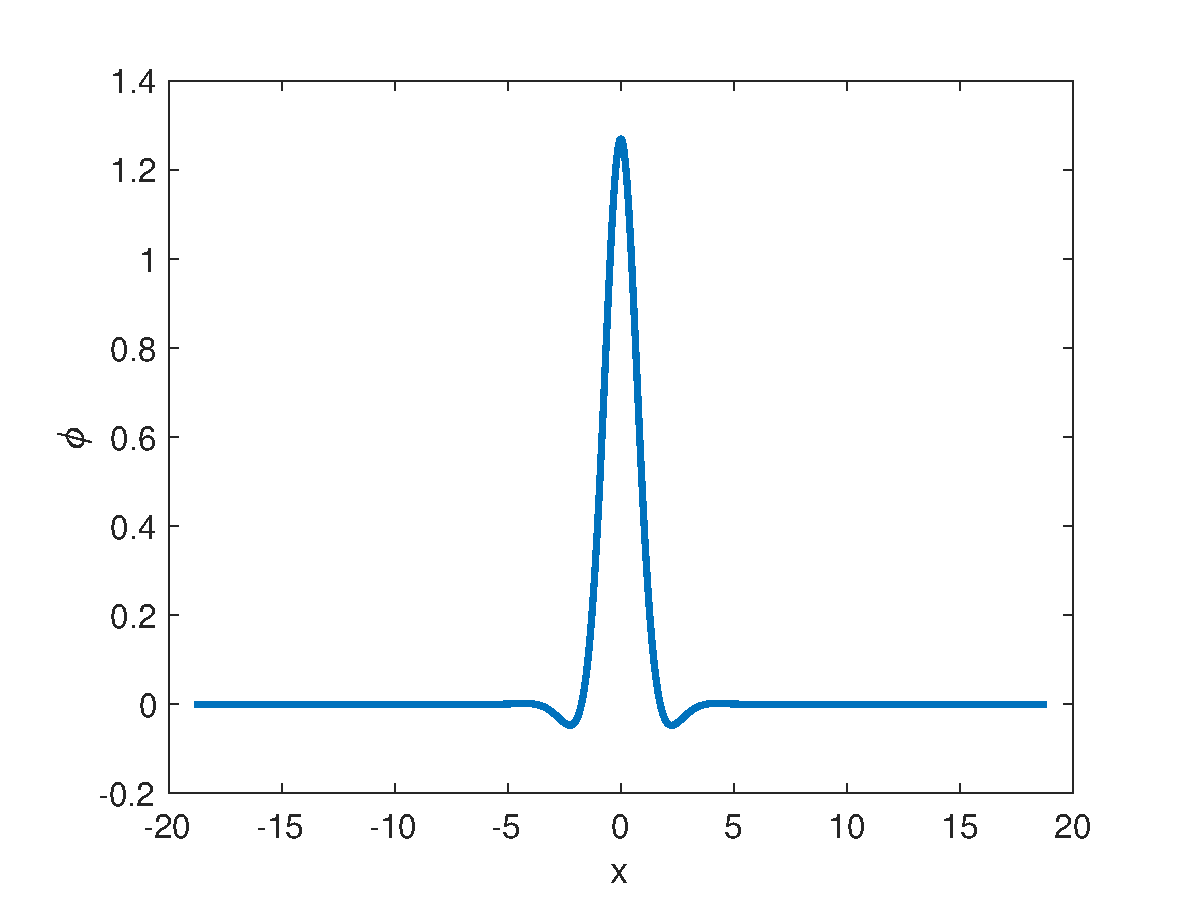
\includegraphics[width=8cm]{images/PQS1.eps} &
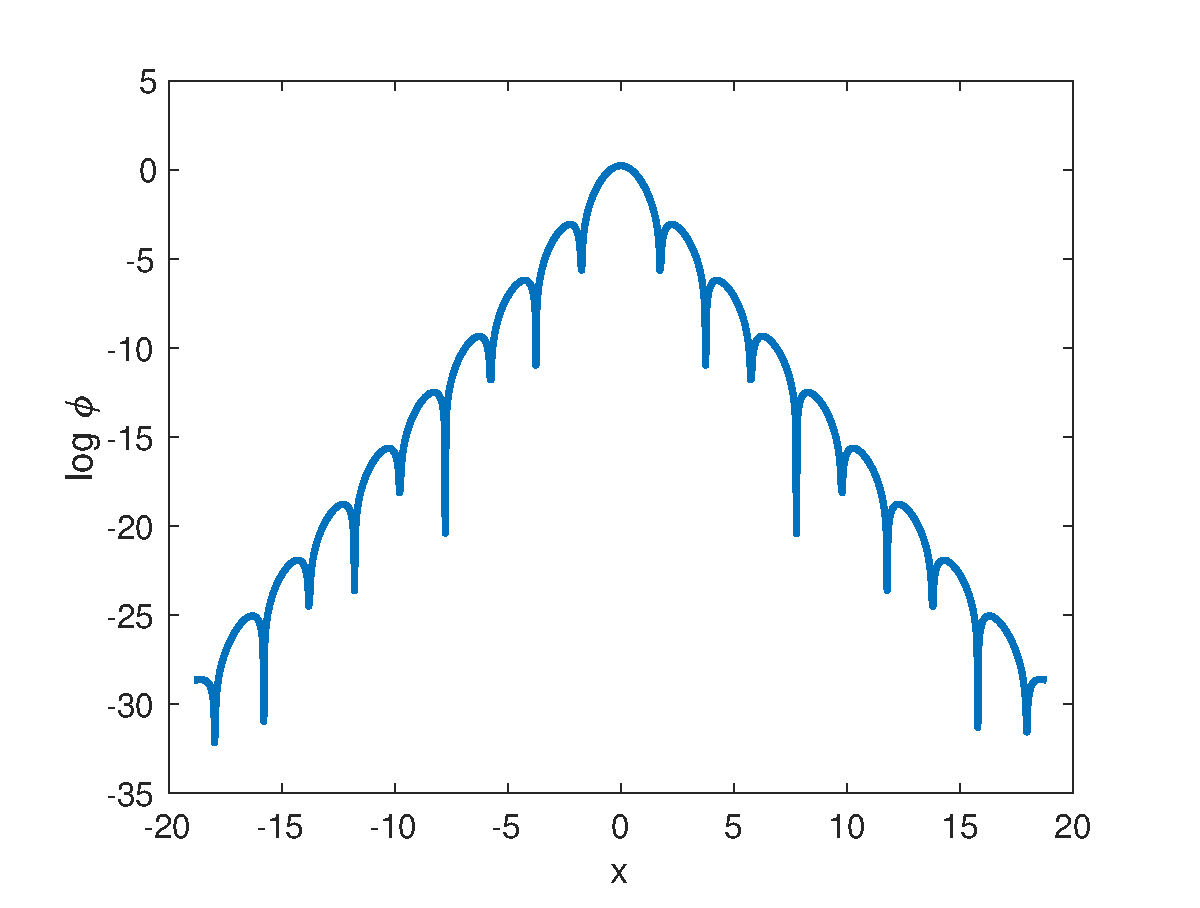
\includegraphics[width=8cm]{images/PQS1log.eps}
\end{tabular}
\caption{Pure quartic solitary wave solution $\phi(x)$ to \cref{standingwavereal} with $\beta_2 = 0$, $\beta_4 = -1$, $\omega = 1$, and $\gamma = 1$. (left panel). Plot of $\log \phi(x)$ vs $x$ (right panel) showing exponentially-decaying oscillatory tails. Spatial discretization is a uniform grid with $N = 1024$ grid points, and we use periodic boundary conditions. }
\label{fig:PQS}
\end{figure} 

To determine the spectrum of the linearization about the primary pulse, we construct the linear operator $\calL(\phi)$ using Fourier spectral differentiation matrices \revised{with periodic boundary conditions} and compute the eigenvalues using Matlab's eigenvalue solver \texttt{eig} (\cref{fig:PQSspec}, left panel). \revised{Since the spectral problem is posed on a periodic domain, the essential spectrum is discrete. It is a finite set of points in this case since spatial discretization approximates the eigenvalue problem \cref{multieig} with an $2N \times 2N$ matrix equation, where $N$ is the number of grid points.} We also note the presence of a pair of internal mode eigenvalues on the imaginary axis.  

\begin{figure}[H]
\centering
\begin{tabular}{cc}
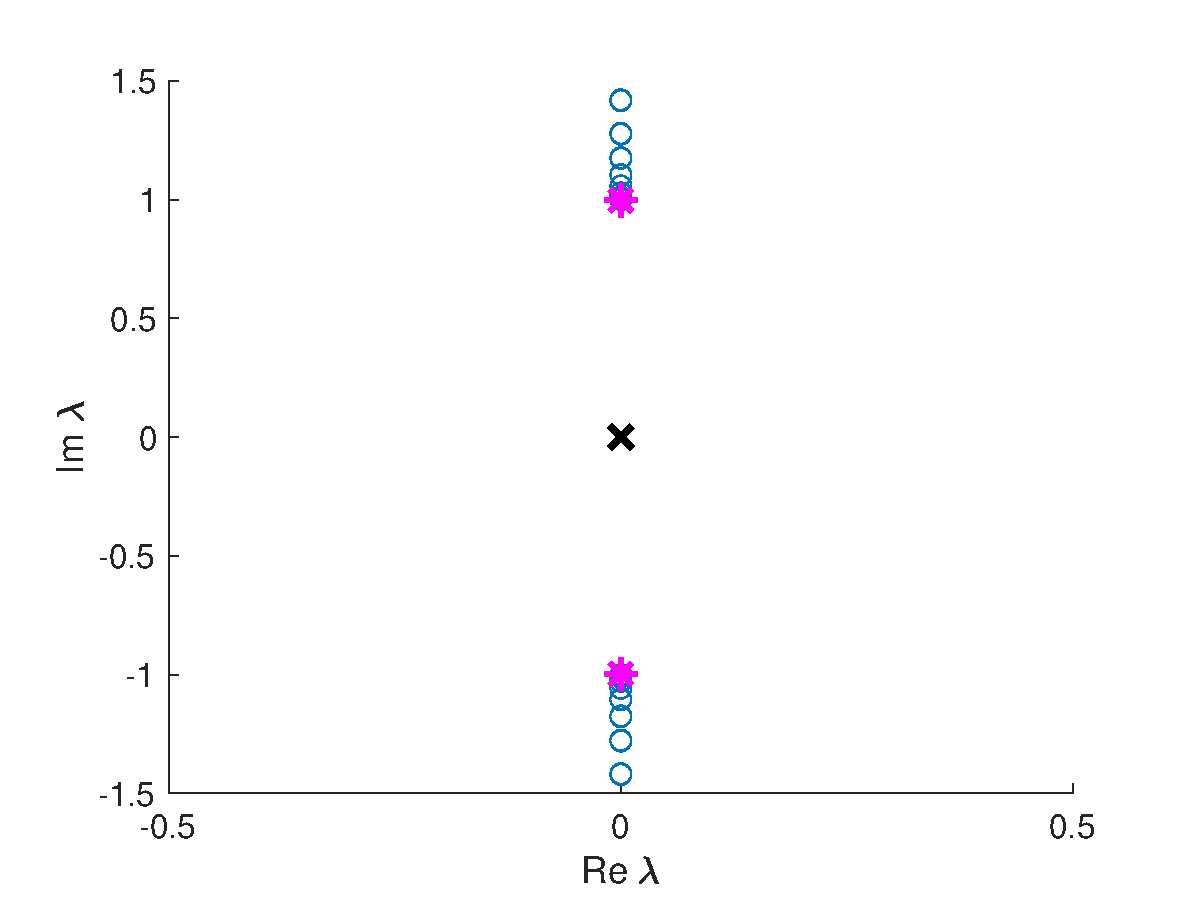
\includegraphics[width=8cm]{images/PQSspec.eps} &
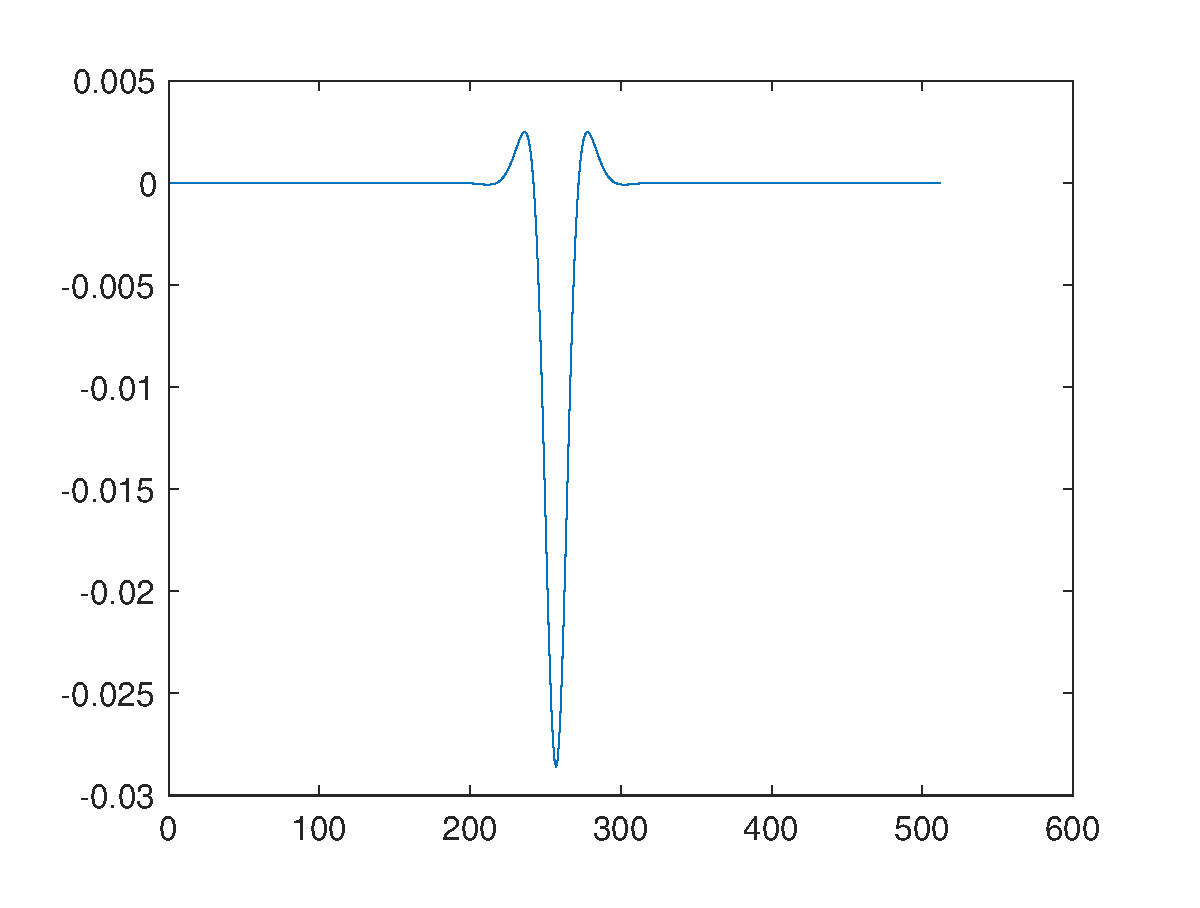
\includegraphics[width=8cm]{images/PQSinternalmode.eps}
\end{tabular}
\caption{Spectrum of pure quartic solitary wave (left panel), $\beta_2 = 0$, $\beta_4 = -1$, $\omega = 1$, and $\gamma = 1$. \revised{Spectrum comprises essential spectrum (blue open circles), internal mode eigenvalues (magenta stars), and kernel eigenvalue with geometric multiplicity 2 and algebraic multiplicity 4 (black X).} Eigenfunction corresponding to internal mode eigenvalue (right panel).}
\label{fig:PQSspec}
\end{figure} 

For the primary solitary wave solutions, we can compute the stability criterion \cref{ddoubleprime} from \cite{Grillakis1987}. In all cases, $M = d''(\omega) > 0$, \revised{thus primary pulse solution is orbitally stable by \cite[Theorem 3.5]{Grillakis1987}}. In addition, numerical computation suggests that $\tilde{M} > 0$.

\subsection{Construction of multipulses}

To construct double pulses, we glue together two copies of the primary pulse at the pulse distances predicted by \cref{theorem:multiexist} and solve for the double pulse solution using the same Newton conjugate-gradient method we used above. The first four double pulse solutions are shown in \cref{fig:doublepulses}. 
\begin{figure}[H]
\centering
\begin{tabular}{cc}
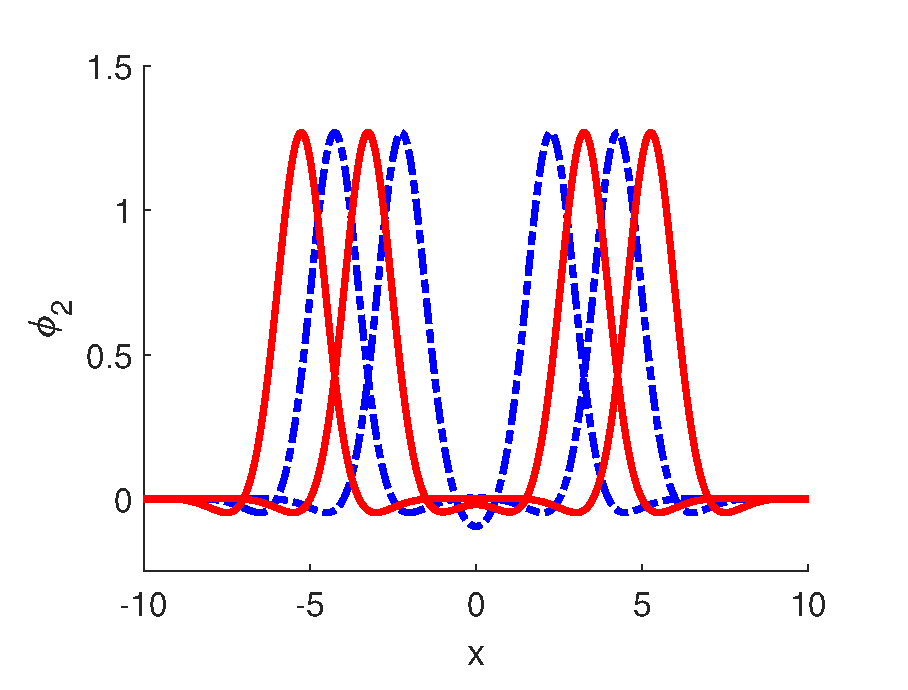
\includegraphics[width=8cm]{images/DPplus.eps} &
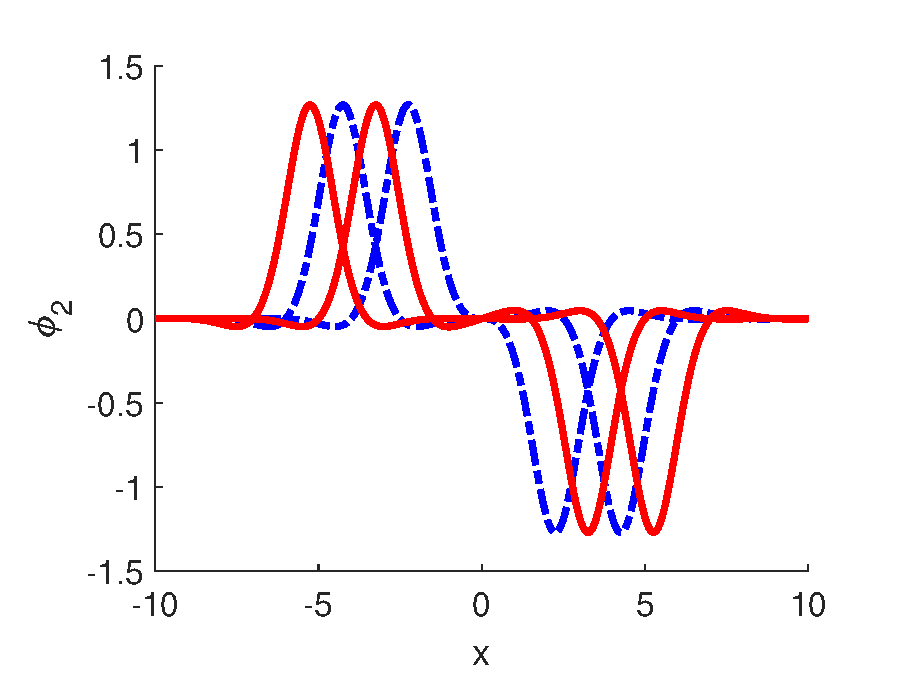
\includegraphics[width=8cm]{images/DPminus.eps}
\end{tabular}
\caption{First four double pulse solutions ($k_1 = 0, 1, 2, 3$) constructed from two pure quartic solitary wave solutions $\phi(x)$ to \cref{standingwavereal}. In-phase double pulses (left panel), opposite phase double pulses (right panel). Dashed blue lines correspond to $k_1$ even, solid red lines correspond to $k_1$ odd. $\beta_2 = 0$, $\beta_4 = -1$, $\omega = 1$, and $\gamma = 1$. }
\label{fig:doublepulses}
\end{figure} 

Arbitrary multi-pulses can similarly be constructed (\cref{fig:triplepulses}). Although the distances between consecutive peaks is constrained by \cref{theorem:multiexist}, these distances do not have to be equal (\cref{fig:triplepulses}, right panel).

\begin{figure}[H]
\centering
\begin{tabular}{cc}
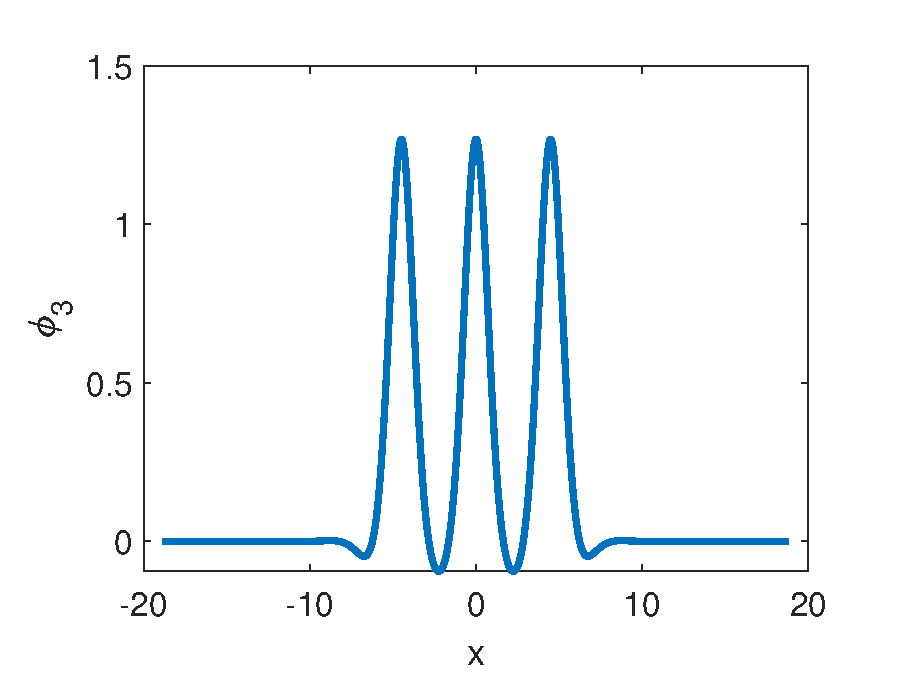
\includegraphics[width=8cm]{images/triple00} &
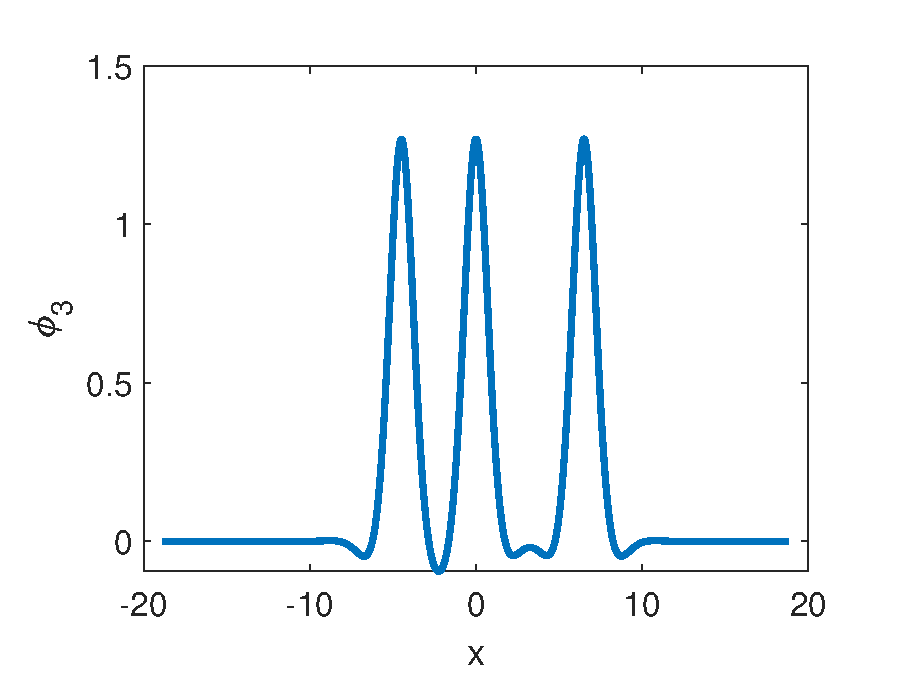
\includegraphics[width=8cm]{images/triple01}
\end{tabular}
\caption{Triple pulse solutions constructed from three pure quartic solitary wave solutions $\phi(x)$ to \cref{standingwavereal}. Symmetric triple pulse with $(k_1, k_2) = (0,0)$ (left panel), asymmetric triple pulse with $(k_1, k_2) = (0,1)$ (left panel). $\beta_2 = 0$, $\beta_4 = -1$, $\omega = 1$, and $\gamma = 1$. }
\label{fig:triplepulses}
\end{figure} 

\subsection{Spectrum of double pulses}

For the spectrum of $\calL(\phi_2)$, the linearization about the double pulse solution $\phi_2$, there is, for both in-phase and out-of-phase double pulses, a pair of purely imaginary interaction eigenvalues $\pm \lambda_i$ and a pair of real interaction eigenvalues $\pm \lambda_r$. This verifies the result of \cref{corr:2pstab} that all double pulses are unstable. \revised{The essential spectrum eigenvalues, as expected, are on the imaginary axis and have magnitude $|\lambda| \geq \omega$. There is also a duplication of the internal mode eigenvalues (\cref{fig:doubleinternalmode}); these appear to be purely imaginary, but they do not affect stability since there is always an interaction eigenvalue with positive real part.}

\begin{figure}[H]
\centering
\begin{tabular}{cc}
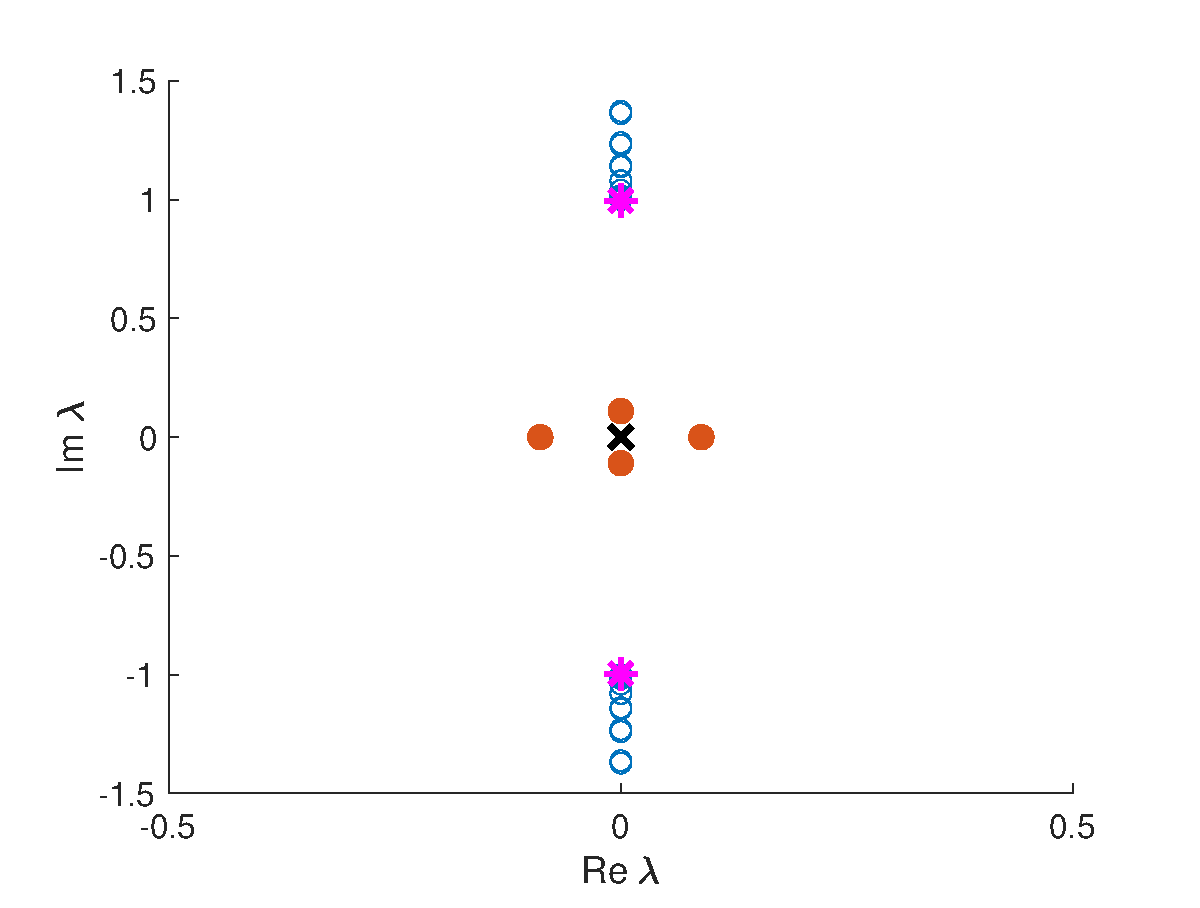
\includegraphics[width=8cm]{images/DP1specpp.eps} &
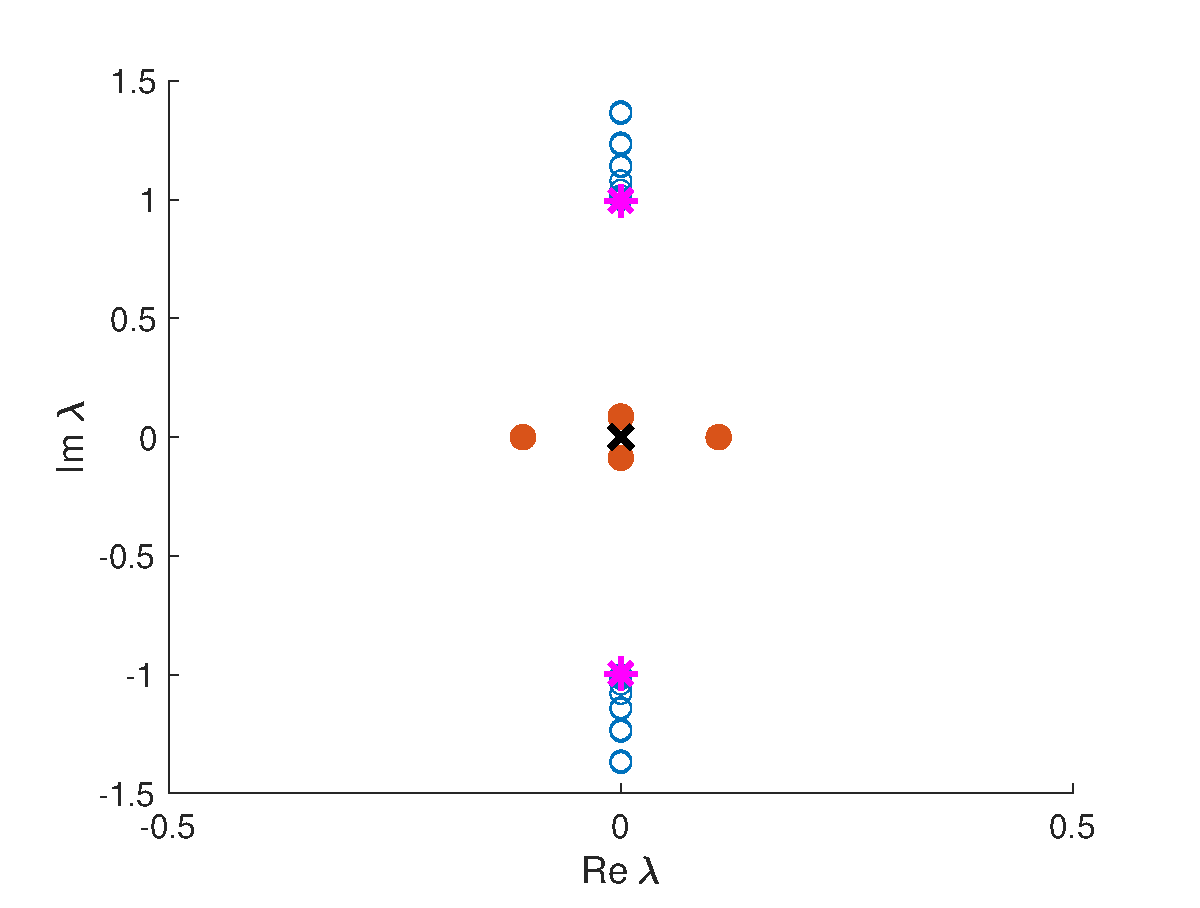
\includegraphics[width=8cm]{images/DP1specmp.eps}
\end{tabular}
\caption{Eigenvalues for first in-phase double pulse (left panel) and first out-of-phase double pulse (right panel). \revised{Spectrum comprises interaction eigenvalues (red dots), essential spectrum (blue open circles), internal mode eigenvalues (magenta stars), and kernel eigenvalue with geometric multiplicity 2 and algebraic multiplicity 4 (black X). See \cref{fig:doublevrvi} for eigenfunctions corresponding to interaction eigenvalues for first in-phase double pulse.} $\beta_2 = 0$, $\beta_4 = -1$, $\omega = 1$, and $\gamma = 1$.}
\label{fig:doublespec}
\end{figure} 

\begin{figure}[H]
\centering
\begin{tabular}{c}
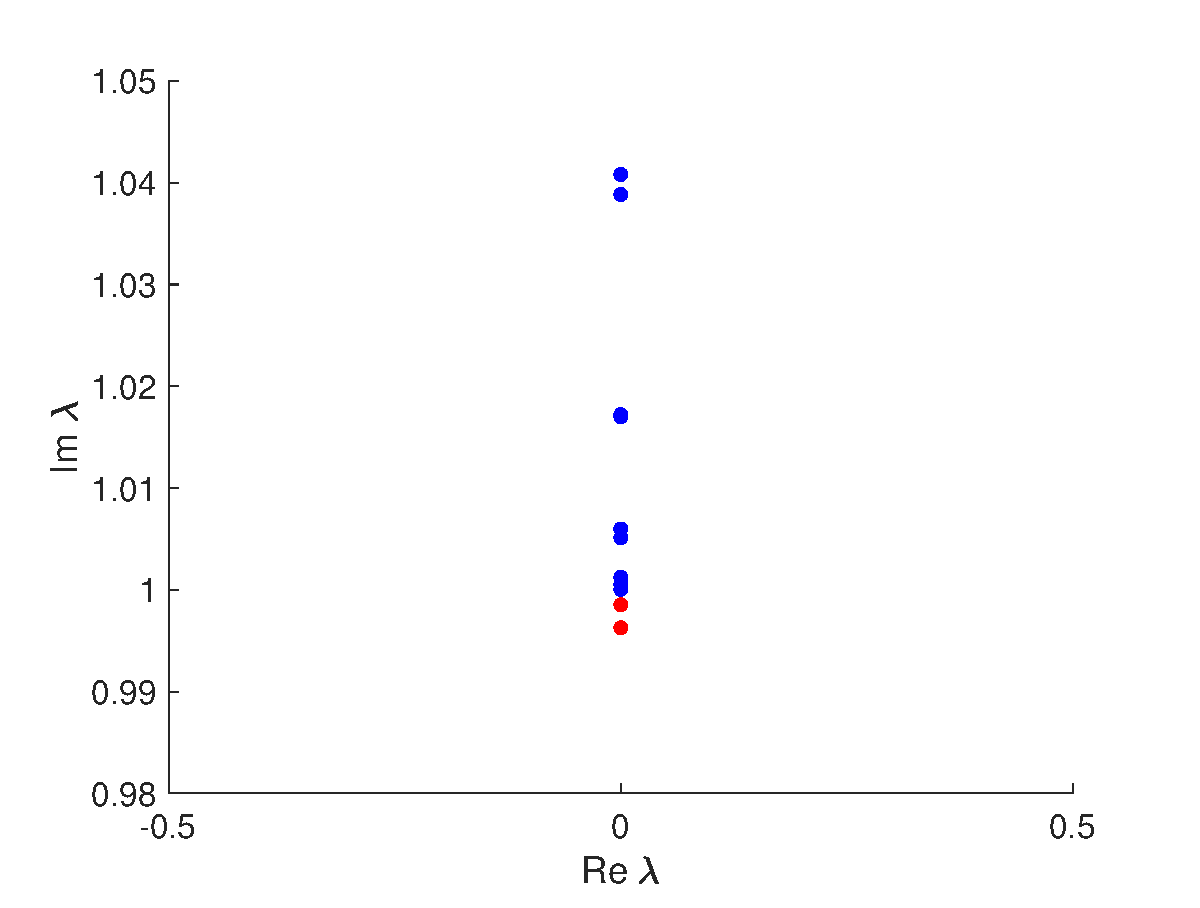
\includegraphics[width=8cm]{images/DP3internalmode.eps}
\end{tabular}
\caption{Close-up of spectrum near $\lambda = i$ showing pair of internal mode eigenvalues (magenta stars) and essential spectrum eigenvalues (blue open circles). Third in-phase double pulse. $\beta_2 = 0$, $\beta_4 = -1$, $\omega = 1$, and $\gamma = 1$.}
\label{fig:doubleinternalmode}
\end{figure}

\revised{For the first in-phase double pulse ($k_1 = 0$), the eigenfunctions $v_r(x)$ and $v_i(x)$ corresponding to the real and imaginary interaction eigenvalue $\lambda_r$ and $\lambda_i$ (respectively) are shown in \cref{fig:doublevrvi}. For in-phase double pulses with $k_1$ even, $v_r(x)$ resembles a linear combination of translates of $(0, \phi)^T$, and $v_i(x)$ resembles a linear combination of translates of $(\partial_x \phi, 0)^T$. (See \cref{sec:proofs} for the construction of these eigenfunctions using Lin's method). This is the same for out-of-phase double pulses with $k_1$ odd, and is reversed for in-phase double pulses with $k_1$ odd and out-of-phase double pulses with $k_1$ even.}

\begin{figure}[H]
\centering
\begin{tabular}{cc}
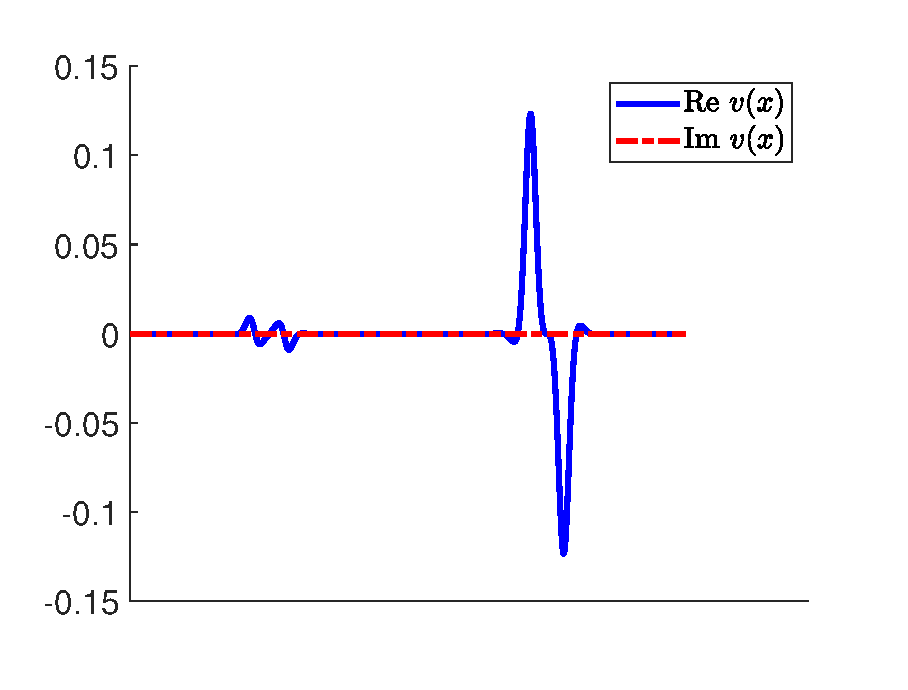
\includegraphics[width=8cm]{images/DP0ppvr} &
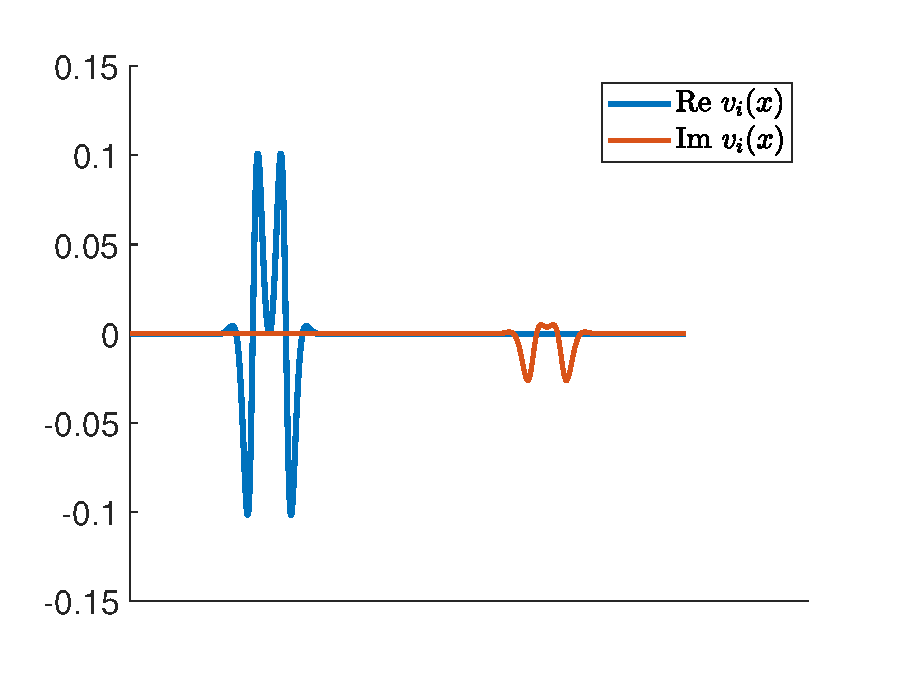
\includegraphics[width=8cm]{images/DP0ppvi}
\end{tabular}
\caption{\revised{Eigenfunction $v_r(x)$ corresponding to $\lambda_r = 0.0891$ (left panel), and real and imaginary parts of eigenfunction $v_i(x)$ corresponding to $\lambda_i = 0.1098i$ (right panel) for first in-phase double pulse $(k_1 = 0)$. $\beta_2 = 0$, $\beta_4 = -1$, $\omega = 1$, and $\gamma = 1$.}}
\label{fig:doublevrvi}
\end{figure}

Finally, we verify the formulas for the interaction eigenvalues from \cref{corr:2pstab} by plotting the log of the relative error between the leading order term in \cref{inteigpred} and the eigenvalues computed by Matlab versus the pulse separation distance $X$ (\cref{fig:inteigpred}). 

\begin{figure}[H]
\centering
\begin{tabular}{c}
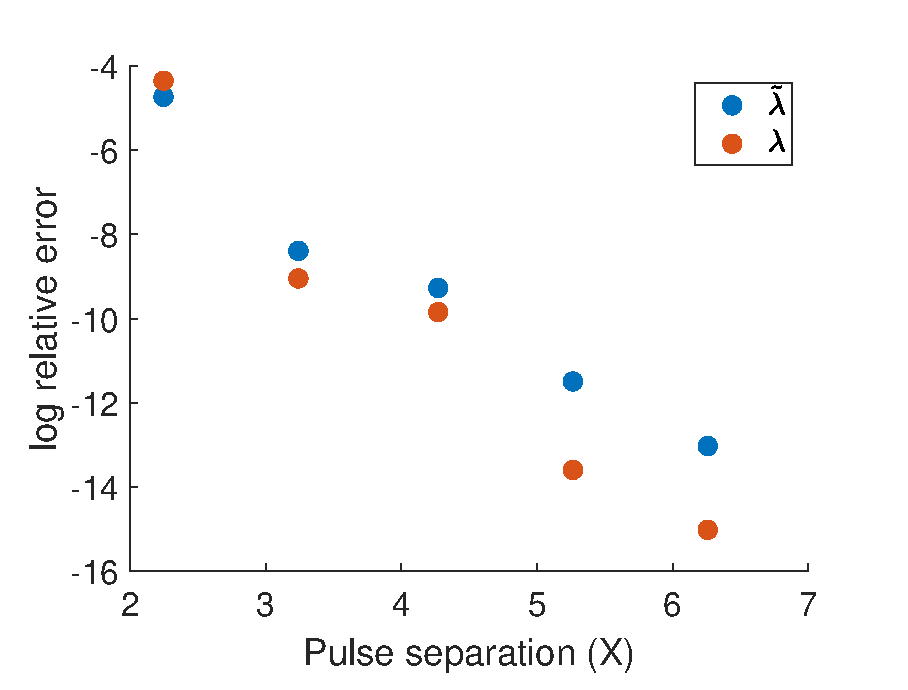
\includegraphics[width=8cm]{images/inteigpred.eps}
\end{tabular}
\caption{Log of the relative error for the eigenvalues $\lambda_\pm$ versus the pulse separation $X$ for the first five in-phase double pulses. $\beta_2 = 0$, $\beta_4 = -1$, $\omega = 1$, and $\gamma = 1$.}
\label{fig:inteigpred}
\end{figure}

\subsection{Timestepping}

We perform numerical timestepping experiments to characterize the nature of the instability for multipulse solutions to \cref{NLS4}. Since the multipulses we constructed above are standing waves with frequency $\omega$, we rewrite \cref{NLS4} in a co-rotating frame as 
\begin{equation}\label{NLS4rot}
u_t = i\left( \frac{\beta_4}{24}u_{xxxx} - \frac{\beta_2}{2}u_{xx} - \omega u + \gamma |u|^2 u \right),
\end{equation}
so that the solutions of interest are equilibrium solutions to \cref{NLS4rot}. For the timestepping scheme, we use a split-step Fourier method \cite{Agrawal2013,Bogomolov2006} 
\[
u(x,t+h) = \calF^{-1} \left\{  e^{i h \left( (\beta_4/24) k^4 - (\beta_2/2)k^2 - \omega \right) } \calF\left( e^{ih |u(x,t)|^2} u(x,t) \right) \right\},
\]
where $h$ is the time step size, $k$ is the frequency in Fourier space, and the Fourier transform $\calF$ is implement using the fast Fourier transform.

For double pulses, given the eigenfunctions we computed in the previous section, we expect to see perturbations evolve either in the distance between the two peaks, corresponding to the eigenfunction resembling copies of $(\partial_x \phi, 0)^T$, or the phase difference between the two peak, corresponding to the eigenfunction resembling copies of $(0, \phi)^T$. (See \cite[Figure 9]{Pelinovsky2007} for timestepping results for double pulses in the 5th order KdV equation; in that case, there is a single continuous symmetry in the underlying system, and perturbations evolve in the distance between the two peaks).

\begin{figure}[H]
\centering
\begin{tabular}{cc}
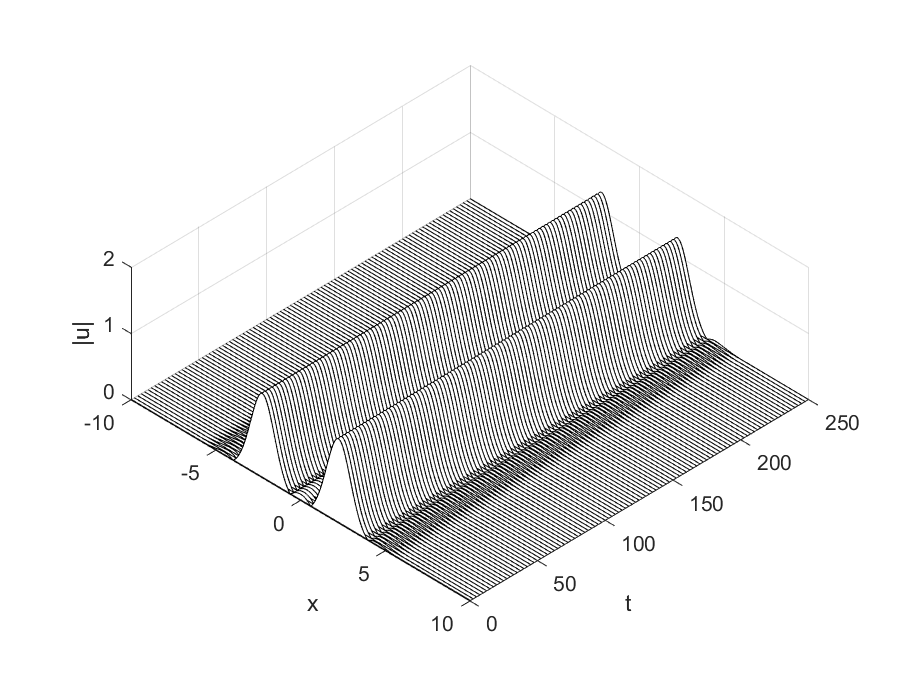
\includegraphics[width=8cm]{images/DP0ppwaterfall} &
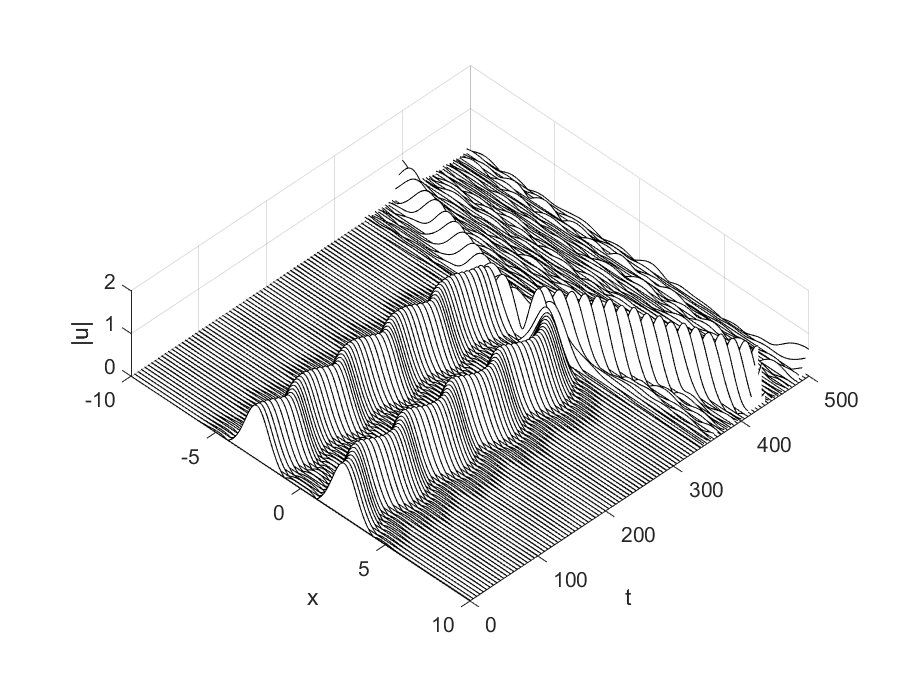
\includegraphics[width=8cm]{images/DP0ppstretchwaterfall} \\
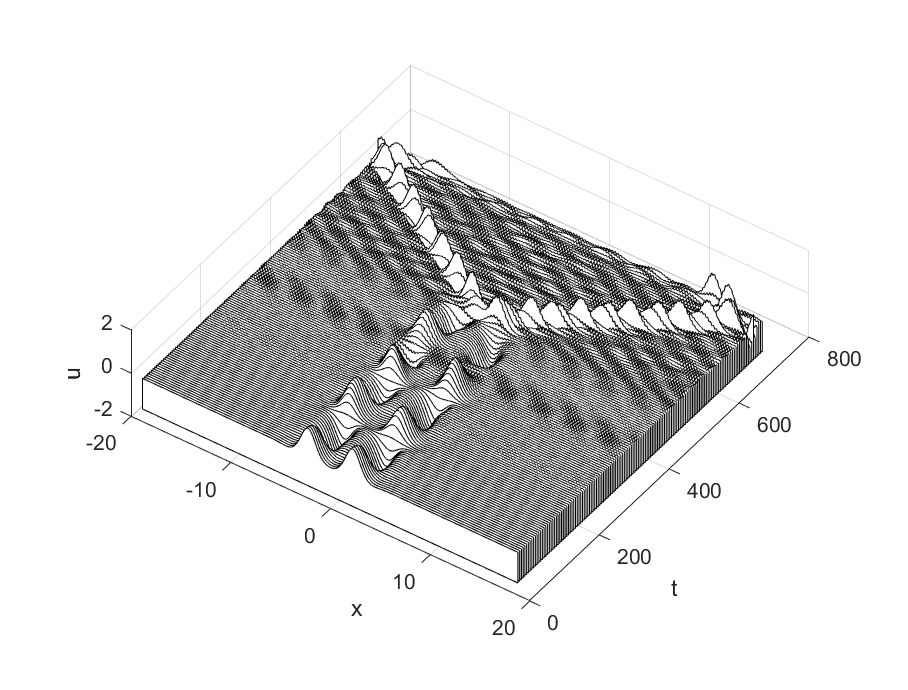
\includegraphics[width=8cm]{images/DP0ppphasewaterfall} &
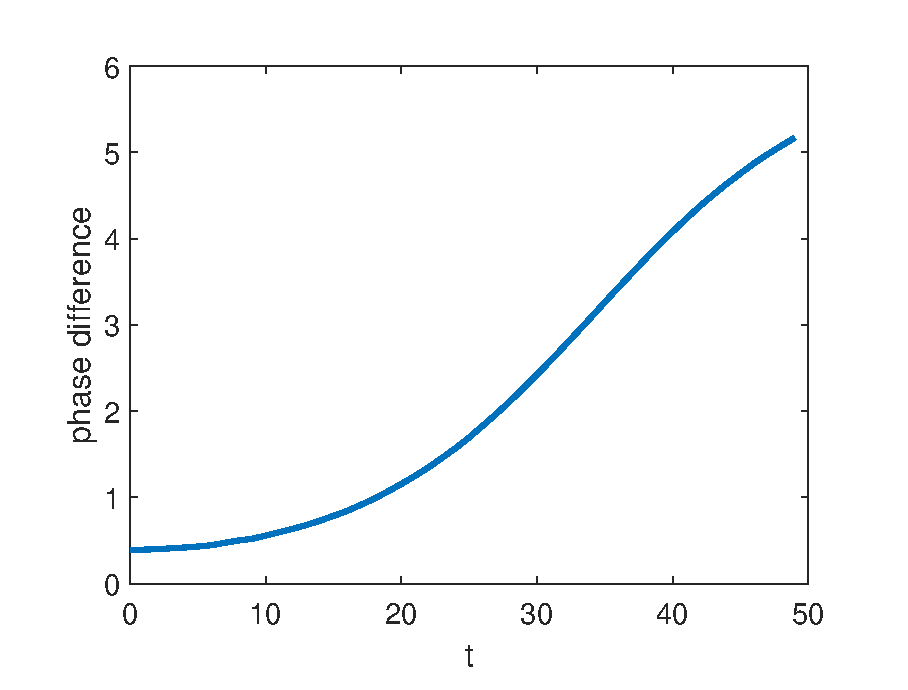
\includegraphics[width=6cm]{images/DP0ppphasedifference}
\end{tabular}
\caption{Hi.}
\label{fig:timestep0pp}
\end{figure}

\begin{figure}[H]
\centering
\begin{tabular}{cc}
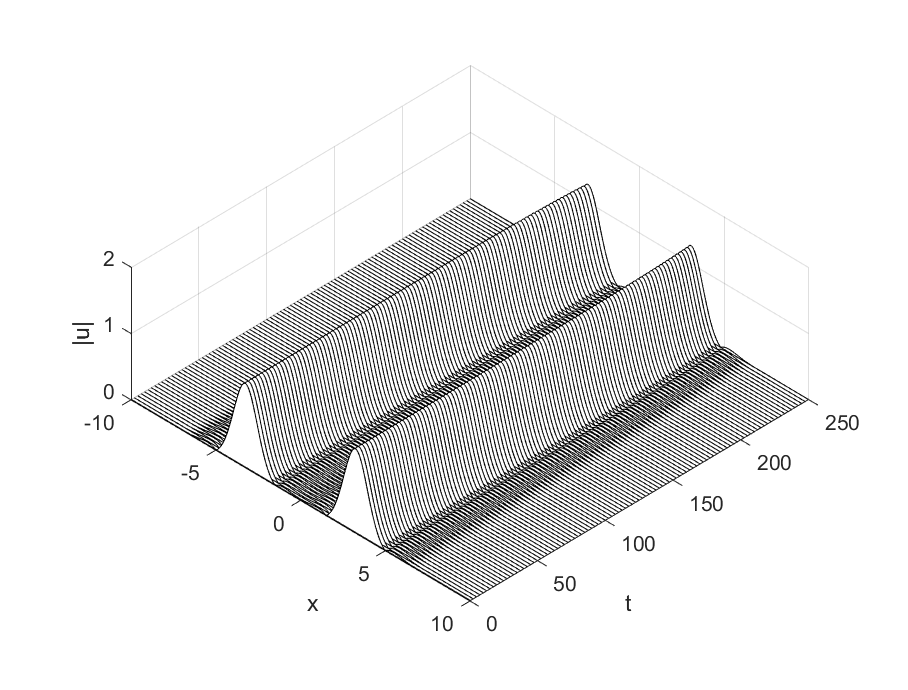
\includegraphics[width=8cm]{images/DP1ppwaterfall} &
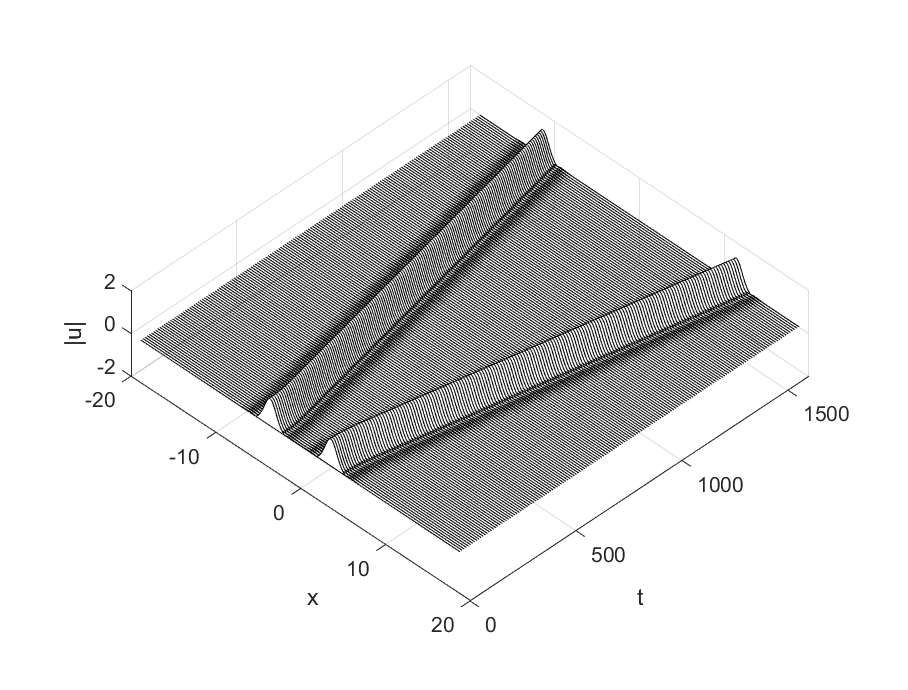
\includegraphics[width=8cm]{images/DP1ppstretchwaterfall} \\
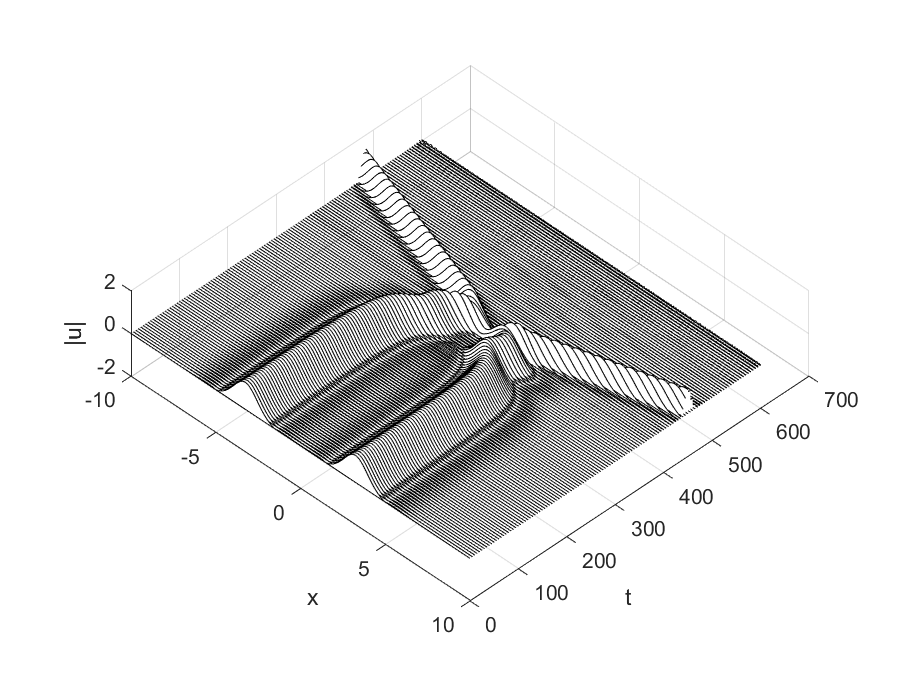
\includegraphics[width=8cm]{images/DP1ppphasewaterfall} &
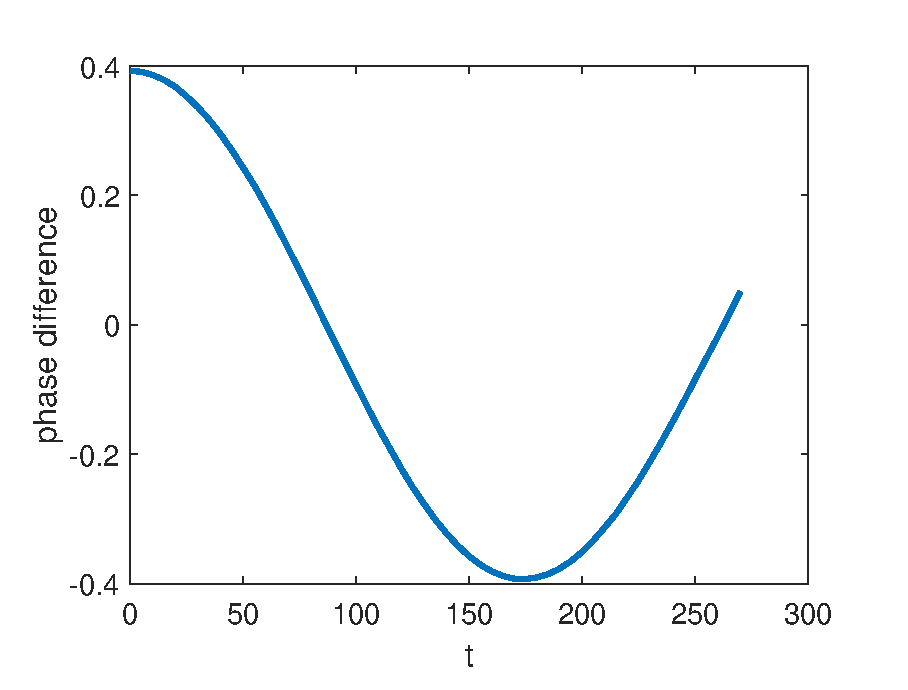
\includegraphics[width=6cm]{images/DP1ppphasedifference}
\end{tabular}
\caption{Hi.}
\label{fig:timestep1pp}
\end{figure}





\section{Conclusions and future directions}

In this paper, we studied single and multi-pulse solitary wave solutions to a general nonlinear Schr{\"o}dinger equation with both second and fourth order dispersion terms. We gave criteria for the existence of a primary soliton solution in terms of the parameters of the system, and provided numerical verification that the primary soliton is orbitally stable. We then constructed $n$-pulse solutions by splicing together multiple copies of the primary pulse, and reduced the problem of finding the small eigenvalues resulting from interaction between neighboring pulses to that of computing the determinant of a $2n\times2n$ block matrix. Under a mild assumption, which can be verified numerically, we showed that all multi-pulse solutions are unstable. For future research, we could investigate solitons and multi-pulses in higher order NLS equations, as discussed in \cite{Runge2020}. We expect that these results would hold for these higher order variants, and that all multi-pulse solutions would be unstable. We could also study generalizations to other nonlinearities. It would be interesting to perform numerical time-stepping starting with perturbed multi-pulses to investigate how the instability evolves in time. Although all multi-pulse solutions to this fourth order model are unstable, this equation represents an idealization of the experimental situation since energy is always conserved. A more realistic model might incorporate gains and losses of energy in the laser cavity, and it is possible that stable multi-pulses could exist in such a scenario.

\section{Proof of stability results}\label{sec:proofs}

\subsection{Proof of Theorem \ref{th:blockmatrix}}\label{sec:blockmatrixproof}

The proof is adapted from \cite[Section 3.4]{Manukian} and the proof of \cite[Theorem 2]{Sandstede1998}, and uses an implementation of the Lyapunov-Schmidt reduction known as Lin's method. It follows from \cref{Lphikernel} that
\begin{equation}\label{Kkernel}
\begin{aligned}
[Y(x)]' &= K(\phi_n)Y(x), \quad [Z(x)]' = K(\phi_n)Z(x) + B_1 Y(x) \\
[\tilde{Y}(x)]' &= K(\phi_n)\tilde{Y}(x), \quad [\tilde{Z}(x)]' = K(\phi_n)\tilde{Z}(x) + B_1 \tilde{Y}(x),
\end{aligned}
\end{equation}
where
\begin{equation}
\begin{aligned}
Y(x) &= ( 0, U_n(x) )^T, \quad
Z(x) = ( \partial_\omega U_n(x), 0 )^T \\
\tilde{Y}(x) &= ( \partial_x U_n(x), 0)^T, \quad
\tilde{Z}(x) = ( 0, Z_n(x) )^T,
\end{aligned}
\end{equation}
$Z_n(x) = (z_n(x), \partial_x z_n(x), \partial_x^2 z_n(x), \frac{\beta_4}{24} \partial_x^3 z_n(x))$, and the first component $z_n(x)$ solves $\calL^-(\phi_n)z_n = \phi_n'$. The analysis is identical to that of \cite{Manukian}, except the piecewise ansatz for the eigenfunction also involves $Z(x)$ and $\tilde{Z}(x)$. Writing the functions \cref{Kkernel} in piecewise form as with \cref{Unpiecewise}, we take the ansatz
\begin{align}\label{Vansatz}
V_i^\pm(x)' &= d_i(Y_i^\pm(x) + \lambda Z_i^\pm(x)) + \tilde{d}_i(\tilde{Y}_i^\pm(x) + \lambda \tilde{Z}_i^\pm(x)) + W_i^\pm && i = 1, \dots, n,
\end{align}
where $V_i^- \in C^0( [-X_{i-1}, 0], \C^8 )$ and $V_i^+ \in C^0( [0, X_i], \C^8 )$. Substituting \cref{Vansatz} into \cref{multieig} and simplifying using \cref{Kkernel}, the remainder functions $W_i^\pm(x)$ solve the equation
\begin{align}\label{Wsolves}
W_i^\pm(x)' &= K(\phi_n)W_i^\pm(x) + \lambda^2 d_i B Z_i^\pm(x) + \lambda^2 \tilde{d}_i B \tilde{Z}_i^\pm(x) && i = 1, \dots, n.
\end{align}
Following \cite{Manukian,Sandstede1998}, we obtain a unique piecewise solution $W_i^\pm(x)$ which generically has $n$ jumps at $x = 0$ in the direction of $Q^*(0) \oplus \tilde{Q}^*(0)$. Using the definitions of $Q^*(x)$ and $\tilde{Q}^*(x)$ together with \cref{Unestimates} and \cite[(3.19)]{Manukian}, these jumps are given by
\begin{equation}\label{jumpcond1}
\begin{aligned}
\xi_i &= \theta_{i+1} \langle \Psi(X_i), U(-X_i) \rangle (d_{i+1} - d_i) 
+ \theta_{i-1} \langle \Psi(-X_{i-1}), U(X_{i-1}) \rangle (d_i - d_{i-1} )  \\
&\qquad + \lambda^2 \theta_i d_i \int_{-\infty}^\infty \langle \Psi(y), B \partial_\omega U(y) \rangle dy 
+ \mathcal{O}((|\lambda| + e^{-\alpha X_{\min}})^3) \\
\tilde{\xi}_i &= \theta_{i+1} \langle \Psi'(X_i), U'(-X_i) \rangle (\tilde{d}_{i+1} - \tilde{d}_i) 
+ \theta_{i-1} \langle \Psi'(-X_{i-1}), U'(X_{i-1}) \rangle (\tilde{d}_i - \tilde{d}_{i-1}) \\
&\qquad- \lambda^2 \theta_i \tilde{d}_i \int_{-\infty}^\infty \langle \Psi(y), B Z(y) \rangle dy 
+ \mathcal{O}((|\lambda| + e^{-\alpha X_{\min}})^3),
\end{aligned}
\end{equation}
where $Z(x) = (z(x), \partial_x z(x), \partial_x^2 z(x), \frac{\beta_4}{24} \partial_x^3 z(x))$. By symmetry, 
\begin{equation}\label{Rrelation}
\Psi(-x) = -R \Psi(x), \quad U(-x) = R U(x),
\end{equation}
where $R$ is the standard reversor operator 
\[
R(u_1, u_2, u_3, u_4) = (u_1, -u_2, u_3, -u_4),
\] 
thus 
\begin{equation}\label{PsiR}
\begin{aligned}
\langle \Psi(-X_{i-1}), U(X_{i-1}) \rangle &= -\langle \Psi(X_{i-1}), U(-X_{i-1}) \rangle \\
\langle \Psi'(-X_{i-1}), U'(X_{i-1}) \rangle &= -\langle \Psi'(X_{i-1}), U'(-X_{i-1}) \rangle.
\end{aligned} 
\end{equation}
Finally, we relate $\langle \Psi(X_i), U(-X_i) \rangle$ and $\langle \Psi'(X_i), U'(-X_i) \rangle$. Since $DF(\phi) = K^+(\phi)$, $\Psi(x)$ is the unique bounded solution to the adjoint equation $W'(x) = -DF(\phi)^* W(x)$. Thus by \cite[Lemma 6.1]{Sandstede1998}, with $\Psi'(x)$ in place of $\Psi(x)$, $p$ in place of $\phi$, and no parameter $\mu$,
\begin{align}
\langle \Psi'(x), U(-x) &= \langle \Psi'(-x), U(x) \rangle = s e^{-2 a x} \sin(2 b x + p) + \mathcal{O}(e^{-(2 \alpha + \gamma)x}) \label{IPdPsiU} \\
\langle \Psi'(x), U'(-x) \rangle &= 
\langle \Psi'(x), U'(-x) \rangle = -s e^{-2 a x} \left( b \cos(2 b x + p) - a \sin(2 b x + p) \right) + \mathcal{O}(e^{-(2 \alpha + \gamma)x}), \label{IPdPsidU}
\end{align}
where $s > 0$ and $\gamma > 0$. Differentiating $\langle \Psi(-x), U(x) \rangle$ with respect to $x$, since the operator $\partial_x$ is skew symmetric, 
\begin{align*}
\frac{d}{dx} \langle \Psi(x), U(-x) \rangle = 2 \langle \Psi'(x), U(-x) \rangle,
\end{align*}
thus we can integrate \cref{IPdPsiU} by parts to get 
\begin{align*}
\langle \Psi(x), U(-x) \rangle = -\frac{1}{a^2 + b^2} s e^{-2 a x} \left( b \cos(2 b x + p) + a \sin(2 b x + p) \right) + \mathcal{O}(e^{-(2 \alpha + \gamma)x}).
\end{align*}
In the proof of \cite[Theorem 3]{Sandstede1998}, the distances $X_i$ are chosen to solve $s e^{-2 a X_i} \sin(2 b X_i + p) = \mathcal{O}(e^{-(2 \alpha + \gamma)X_i})$, thus for $x = X_i$ we have
\begin{align}\label{IPrelation1}
\langle \Psi'(X_i), U'(-X_i) \rangle = (a^2 + b^2)
\langle \Psi(X_i), U(-X_i) \rangle + \mathcal{O}(e^{-(2 \alpha + \gamma)X_i}).
\end{align}
Using \cref{IPrelation1} and \cref{PsiR}, multiplying by $\theta_i$, and using the definition of $B$, equations \cref{jumpcond1} simplify to the jump conditions
\begin{align*}
\xi_i &= \theta_i \theta_{i+1} \langle \Psi(X_i), U(-X_i) \rangle (d_{i+1} - d_i) 
- \theta_{i-1} \theta_i  \langle \Psi(X_{i-1}), U(-X_{i-1}) \rangle (d_i - d_{i-1}) \\
&\qquad + \lambda^2 d_i \int_{-\infty}^\infty \phi(y) \partial_\omega \phi(y) dy 
+ \mathcal{O}( |\lambda|(|\lambda| + e^{-\alpha X_{\min}})^2 + e^{-(2 \alpha + \gamma)X_{\min} }) )  \\
\tilde{\xi}_i &= (a^2 + b^2) \theta_i \theta_{i+1} \langle \Psi(X_i), U(-X_i) \rangle (\tilde{d}_{i+1} - \tilde{d}_i)
- (a^2 + b^2) \theta_{i-1} \theta_i \langle \Psi(X_{i-1}), U(-X_{i-1}) \rangle (\tilde{d}_i - \tilde{d}_{i-1}) \\
&\qquad- \lambda^2 \tilde{d}_i \int_{-\infty}^\infty \partial_y \phi(y) z(y) dy
+ \mathcal{O}( |\lambda|(|\lambda| + e^{-\alpha X_{\min}})^2 + e^{-(2 \alpha + \gamma)X_{\min} }) ) ,
\end{align*}
which we write in matrix form as in the statement of the theorem.

\subsection{Proof of Corollary \ref{corr:multiunstable} and Corollary \ref{corr:2pstab}}

For \cref{corr:multiunstable}, let $\{ \mu_1,\dots,\mu_{n-1}, 0\}$ be the eigenvalues of $A$, which are real and distinct as in the proof of \cite[Theorem 5]{Parker2020}. Following the steps in that proof and using the rescaling in \cite[Theorem 3]{Sandstede1998}, there are $2(n-1)$ pairs of interaction eigenvalues, given by \cref{inteigs}, which are either real or purely imaginary by Hamiltonian symmetry. Since $M > 0$ by \cref{hyp:dccpos}, if $\tilde{M} > 0$ as well, then one of each pair $\lambda_i, \tilde{\lambda}_i$ is real and the other is purely imaginary. \cref{corr:2pstab} is the specific case $n = 2$, where the nonzero eigenvalue of $A$ can be computed directly.

\paragraph{Acknowledgments}

This material is based upon work supported by the U.S. National Science Foundation under the RTG grant DMS-1840260 (R.P. and A.A.).

\bibliography{NLS4.bib}

\end{document}